%\documentclass[11pt,titlepage]{article}
\documentclass[journal=jctcce,manuscript=article]{achemso}
\usepackage[utf8]{inputenc}
%\usepackage[margin=1.0in]{geometry}
\usepackage{graphicx}
\usepackage{subfigure}
\usepackage{amssymb,amsfonts,amsmath}
\usepackage{url}
\usepackage{booktabs, multicol, multirow}
%\usepackage[round,numbers,sort&compress]{natbib}

% Bibliography style (requires the style file biophysj.bst in the 
% document directory)
%\bibliographystyle{biophysj}


\iffalse
\author{Kyle A. Beauchamp, \\
Biophysics Program, \\
Stanford University, Stanford, CA
\and Vijay S. Pande, \\
Chemistry Department and Structural Biology Program, \\
Stanford University, Stanford, CA
\and Rhiju Das \\
Biochemistry and Physics Departments, \\
Stanford University, Stanford, CA
}
\fi

\author{Kyle A. Beauchamp}
\affiliation[Biophysics Program]{Biophysics Program}

\author{Vijay S. Pande$^\dagger$}
\affiliation[Chemistry Department]{Chemistry Department, Stanford University, Stanford, CA}

\author{Rhiju Das$^\dagger$}
\affiliation[Biochemistry Department]{Biochemistry Department, Stanford University, Stanford, CA}


\email{pande@stanford.edu, rhiju@stanford.edu}

\title{Inferring Structural Ensembles from Noisy Experiments and Molecular Dynamics: Correcting Force Field Bias with Bayesian Energy Landscape Tilting}

\begin{document}

\maketitle

\begin{abstract}

Inferring biomolecular conformation from experiment is a fundamental goal of structural biology.  Structure determination often requires the combination of modeling and experiment, but the vast majority of approaches model only a single conformation, provide limited uncertainty information, and inherit biases from assumed force fields when data are limited.  Building on recent conceptual advances, we hypothesized that these biases and missing uncertainty estimates could be addressed through Bayesian Energy Landscape Tilting (BELT), a scheme that enables the systematic computation of fully Bayesian 'hyperensembles' over conformational ensembles.  As a test of BELT's ability to correct force field bias, we show that conformational ensembles of trialanine derived from five different force fields (ff96, ff99, ff99sbnmr-ildn, CHARMM27, and OPLS-AA) and chemical shift and scalar coupling measurements give convergent values of the peptide's $\alpha$, $\beta$, and $PP_{II}$ conformational populations. Furthermore, 
the ensembles recover set-aside measurements not used in the fitting. BELT's principled combination of simulation and limited experimental data promises rigorous assessment of force field bias and sets a foundation for modeling ensembles and uncertainties in complex biomolecular systems.   

\end{abstract}

\emph{Key words:} Molecular Dynamics, NMR, Conformational Ensembles,  Bayesian Statistics

\section*{Introduction}

Over the past forty years, structural biologists have solved ``ground-state'' structures of countless biological macromolecules \cite{Berman2000}. Modern biology, however, presents many systems that do not fit the single-structure paradigm.  "Excited" conformational states of nucleic acids \cite{dethoff2012}, natively disordered proteins \cite{fink2005}, and protein folding intermediates \cite{korzhnev2004} alike are poorly described by single conformation models.  For such systems, models of conformational ensembles are required to understand and predict structural and equilibrium properties.  

A growing body of research has sought to characterize structural ensembles.  Much of it has focused on incorporating dynamical information during NMR structure determination  \cite{lindorff2005simultaneous, lange2008recognition} or the extraction of multiple conformers from X-ray diffraction data  \cite{depristo2004heterogeneity, lang2010automated}.  While these techniques are powerful, they share difficulties in data collection, the unified treatment of heterogeneous experimental data, and the data sparseness relative to the number of degrees of freedom.  In particular, conformational ensemble modeling requires the estimation of not just a single structure, but a collection of structures and their associated equilibrium populations.  This highly under-determined problem involves the simultaneous estimation of approximately $3 \times N \times m$ parameters, where $m$ is the number of states in the ensemble and $N$ is the number of atoms in the molecule.  Inference in this regime necessarily requires 
additional information, which can be provided by combining measurements with simulations performed in an atomistic force field.  

Unfortunately, simulation benchmark studies have demonstrated continuing inaccuracies in molecular dynamics force fields \cite{best2008, lindorff2012systematic, beauchamp2012protein}.  Force field modifications based on direct fitting to NMR measurements have also been demonstrated \cite{li2011iterative, best2012optimization, nerenberg2011}, but such work has optimized only a small fraction of the required force field parameters.  Thus, simulations are often unable to fully recapitulate the wide variety of measurements available on molecular systems.  This inaccuracy poses a challenge when one desires atomic-scale models that are both consistent with presently available measurements and predictive of those yet to be measured.  

Here, we introduce a statistical approach to modeling solution ensembles of biological macromolecules.  The algorithm, Bayesian Energy Landscape Tilting (BELT), uses solution experiments to reweight a collection of atomistic models.  BELT extends a recent maximum entropy method for restraining simulations  \cite{chodera2012} to reweight existing simulations.  Furthermore, BELT leverages Markov Chain Monte Carlo \cite{patil2010pymc} to transform experimental ambiguity into error bars on arbitrary structural features.  BELT modeling produces a hyperensemble or an ``ensemble of ensembles''; the output of BELT is a collection of statistical samples, each of which is a conformational ensemble. 

BELT allows the full characterization of posterior distributions using MCMC.  Most previous approaches, however, have focused on obtaining estimates of a single best-fit conformational ensemble  \cite{rozycki2011saxs,  Graf2007}.  In many cases, however, ambiguous experimental data preclude such a point-estimate of the conformational ensemble.  For example, we plot one measured  \cite{Graf2007} value of $^3J(H_NH^\alpha)$ in the context of the Karplus \cite{vogeli2007limits} equation relating $\phi$ to $^3J(H_NH^\alpha)$.  The measured coupling corresponds to four different values of $\phi$ (Fig. \ref{figure:Ambiguity}a), showing that a point estimate can be inappropriate for modeling conformations.  As previously stated, a point estimate of conformational ensembles is even more ill-posed.  In such cases, it is most appropriate to report a collection of ensembles that are consistent with the available measurements (Fig. \ref{figure:Ambiguity}b).  The BELT approach offers a practical recipe for describing 
such a hyperensemble, computing the hyperensemble's predictions for new experimental observables, and giving error estimates on these predictions.

\begin{figure}
\subfigure[]{
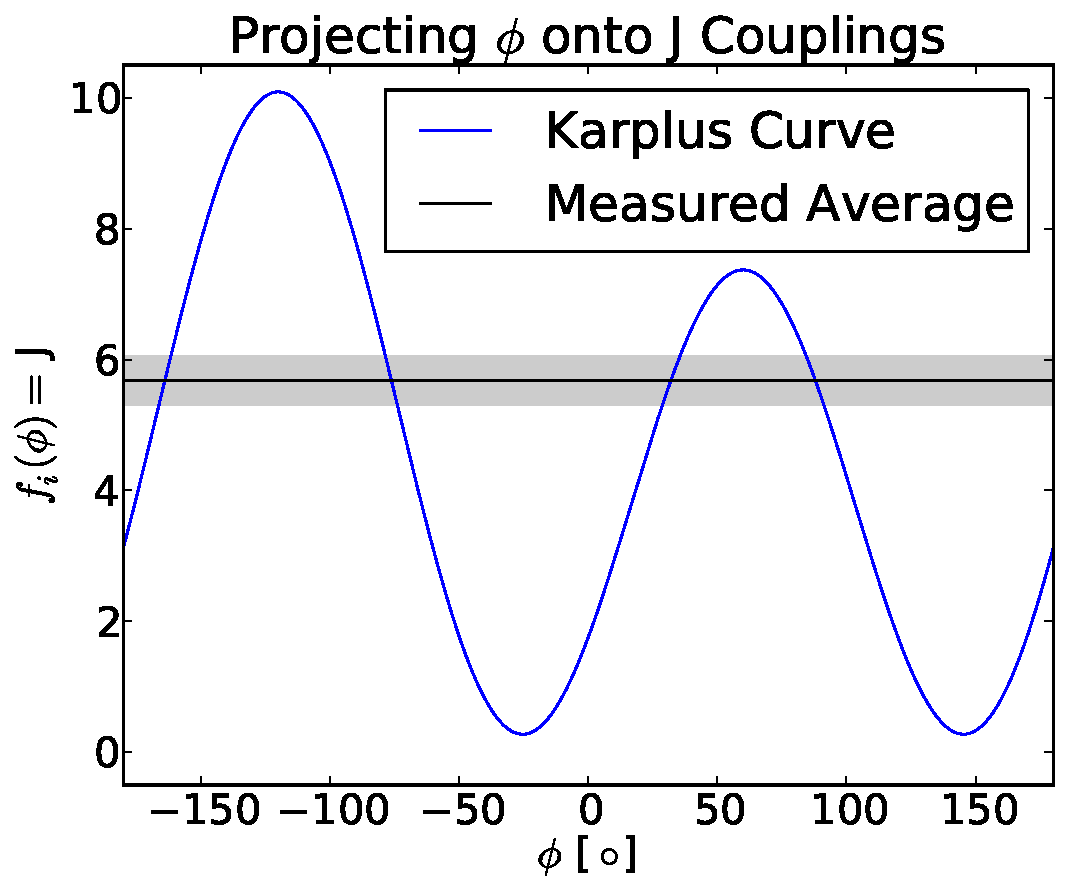
\includegraphics[height=6.25cm]{figures/single_karplus.pdf}
}
\subfigure[]{
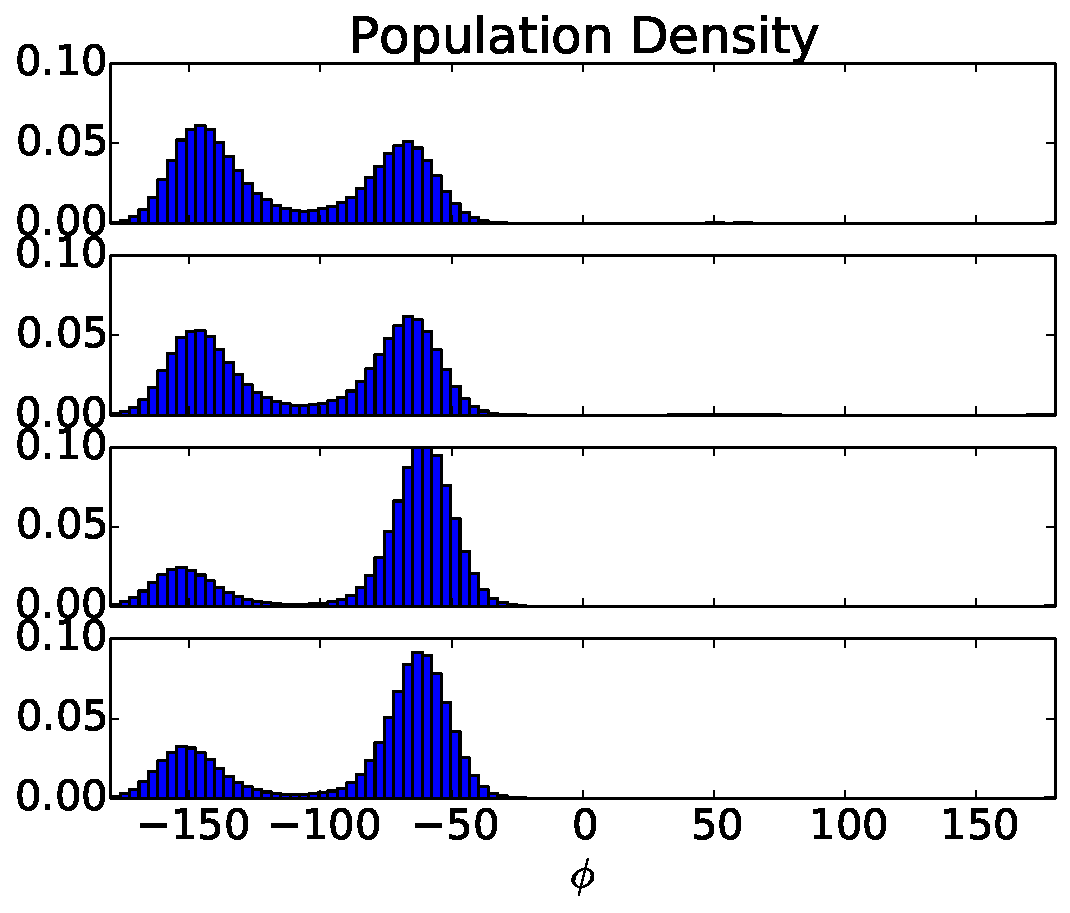
\includegraphics[height=6.25cm]{figures/four_phi_histograms.pdf}
}
\caption{
(a).  The Karplus equation connecting the backbone torsion $\phi$ to $^3J(H_NH^\alpha)$ is ambiguous; the observed value of $^3J(H_NH^\alpha)$ is consistent multiple conformations.  (b).  Four conformational ensembles that fit the data; each ensemble was randomly sampled using BELT as detailed below.  The uncertainty ($\sigma$) on $^3J(H_NH^\alpha)$ was increased 2.5-fold to better illustrate differences.
}
\label{figure:Ambiguity}

\end{figure}


One stringent test of BELT is to assess the convergence of ensembles constructed from force fields with radically different properties.  We therefore investigated the conformational propensities of trialanine using NMR measurements \cite{Graf2007} and MD simulations performed in five different force fields.  The small size of this model system enabled assessment of BELT without complications from incomplete sampling.  At the same time, trialanine populates multiple conformational states and allows a powerful illustration of ensemble modeling.  Although the raw simulations show wide variations in their conformational preferences, BELT corrects force field errors to provide self-consistent estimates of the $\alpha$, $\beta$, and $PP_{II}$ populations.  The ability to correct the biases of diverse forcefields provides a stringent and foundational test of the BELT approach for connecting simulation and equilibrium measurements. 


\section*{Theory: Bayesian Energy Landscape Tilting}

\subsection*{Model Inputs}

To model an ensemble using BELT requires three components (Fig. \ref{figure:BELT}).  First, we need conformations $x_j$  $(j = 1 , ... , m)$ sampled from the equilibrium distribution of some physically realistic model.  This model will serve as a prior on structural properties; in the absence of experimental data, the BELT model inherits the properties of the conformations $x_j$.  In the present work, such conformations will be generated from molecular dynamics simulations.  Second, we require equilibrium experimental measurements $F_i$ $(i = 1 , ... , n)$ and their associated uncertainties $\sigma_i$ $(i = 1 , ... , n)$.  Third, it is necessary to have a direct connection between simulation and experiment.  This connection is achieved by predicting each experimental observable at each conformation: $f_i(x_j)$ is the predicted value of experiment $i$ at conformation $x_j$.  

\begin{figure}

\includegraphics[width=16.0cm]{figures/info_graphic/info_graphic.png}

\caption{
General scheme for BELT modeling.
}
\label{figure:BELT}
\end{figure}

\subsection*{Reweighting}

The next step in constructing an ensemble is to calculate the population of each conformation.  Inspired by a previous method for restraining simulations  \cite{chodera2012} (see Appx. S1), we reweight individual conformations by a biasing potential that is a linear combination of the predicted observables:

$$\Delta U(x;\alpha) = \sum_{i=1}^n \alpha_i f_i(x)$$

In $\Delta U(x;\alpha)$, the parameters $\alpha_i$ determine how strongly each experiment contributes to the biasing potential.  As shown previously \cite{chodera2012}, such a linear biasing potential gives a maximum entropy ensemble for some set of experimental observations. The BELT strategy is to look beyond the single best such ensemble so as to estimate the uncertainty in the ensemble modeling. BELT instead samples over a distribution of such maximum entropy ensembles each parametrized by $\alpha_i$. This approach is connected (see Appx. S1) to prior work by Crooks that proposed an entropic prior for modeling hyperensembles in general physical problems. 

The end result is a collection of `landscape-tilted' ensembles. That is, each conformational ensemble is a perturbed version of the initial molecular dynamics ensemble but reweighted (see Appx. S2) according to energetic perturbations that are linear in the experimental observables $f_i(x)$:

$$\pi_j(\alpha) = \frac{1}{\sum_k \exp[-\Delta U(x_k;\alpha)]} \exp[-\Delta U(x_j;\alpha)]$$

It is informative to consider the case of a single observable $f_1(x)$ (and therefore a single parameter $\alpha_1$).  Suppose the molecule of interest shows a bimodal observable with two equally populated states.  If we let $\alpha_1$ = 0, then the biasing potential is $0$ everywhere and our reweighted ensemble simply returns the results of the MD simulation (Fig. \ref{figure:Hist}b).  If we let $\alpha_1 = -1$, conformations with large values of $f_1(x)$ are upweighted, while conformations with lower values of $f_1(x)$ are downweighted (Fig. \ref{figure:Hist}a).  Finally, if $\alpha_1 = 1$, the ensemble shifts in the opposite direction (Fig. \ref{figure:Hist}c).  

\begin{figure}

\subfigure[]{
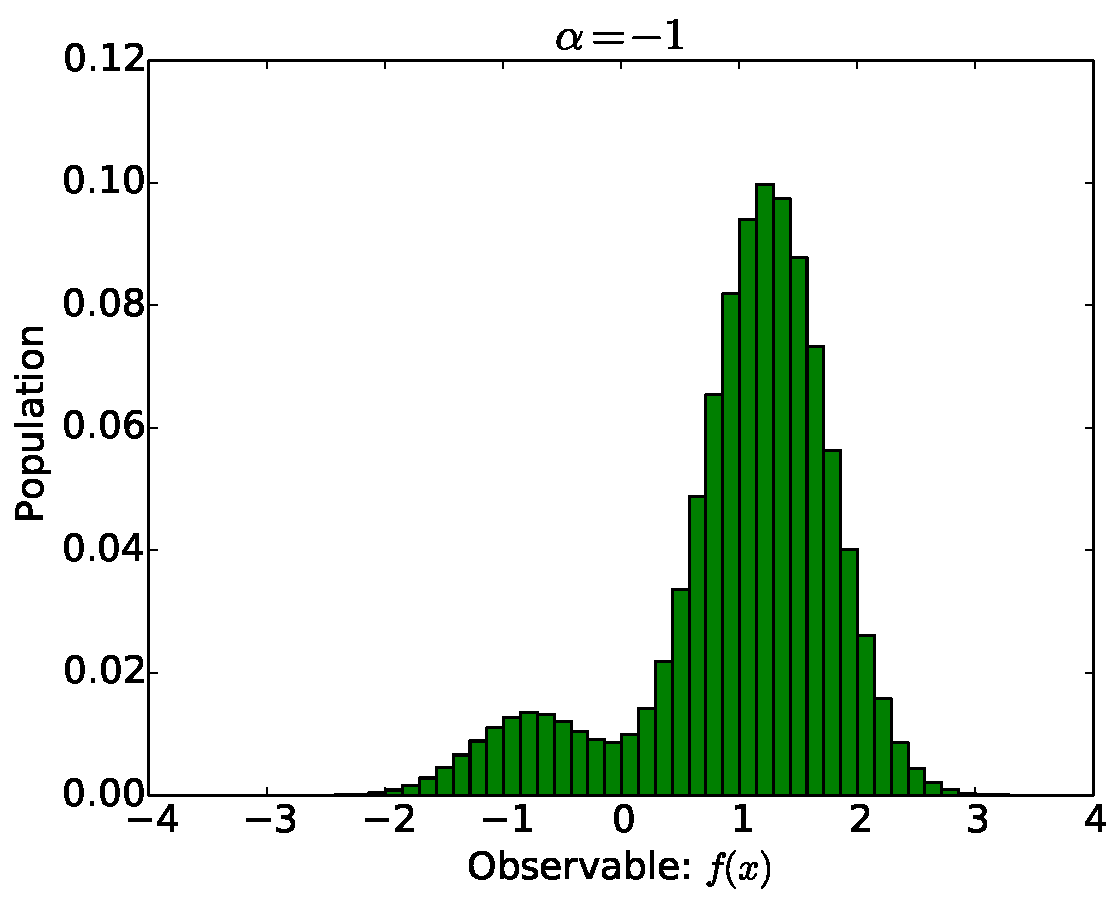
\includegraphics[width=5.0cm]{figures/model_hist-1.pdf}
}
\subfigure[]{
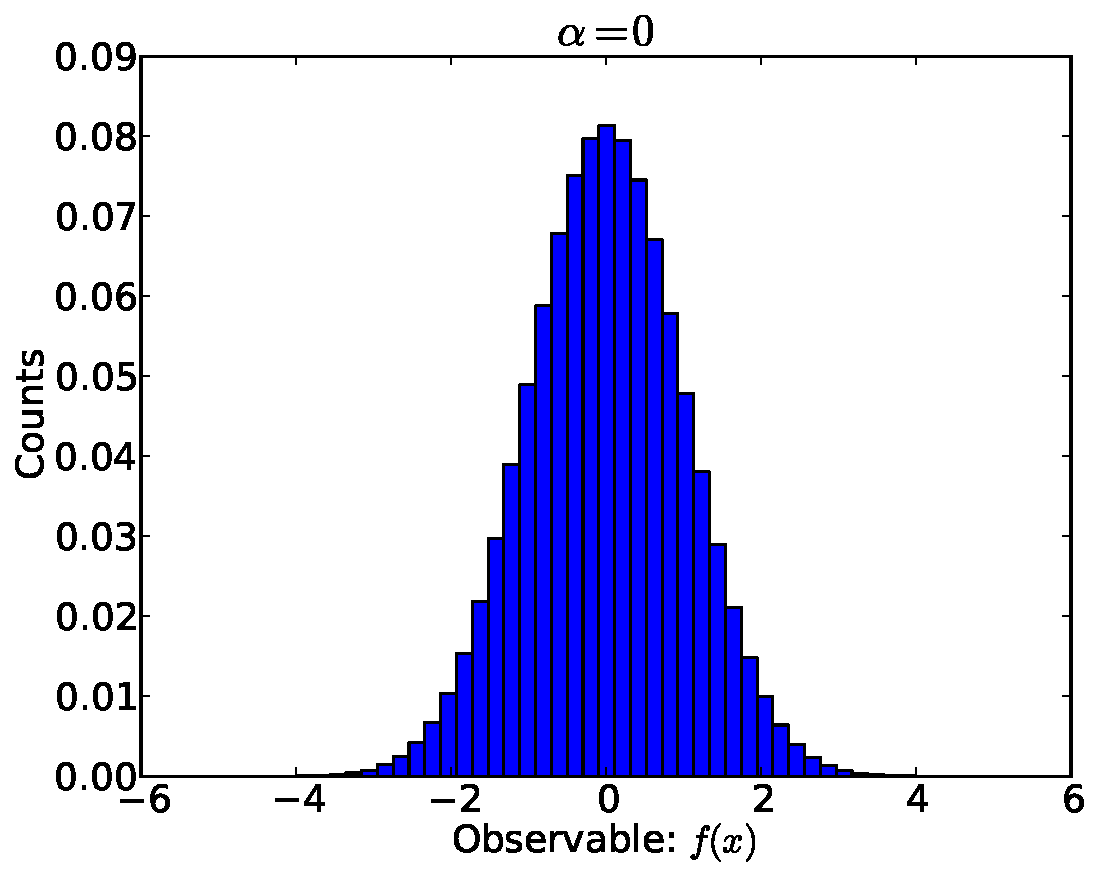
\includegraphics[width=5.0cm]{figures/model_hist0.pdf}
}
\subfigure[]{
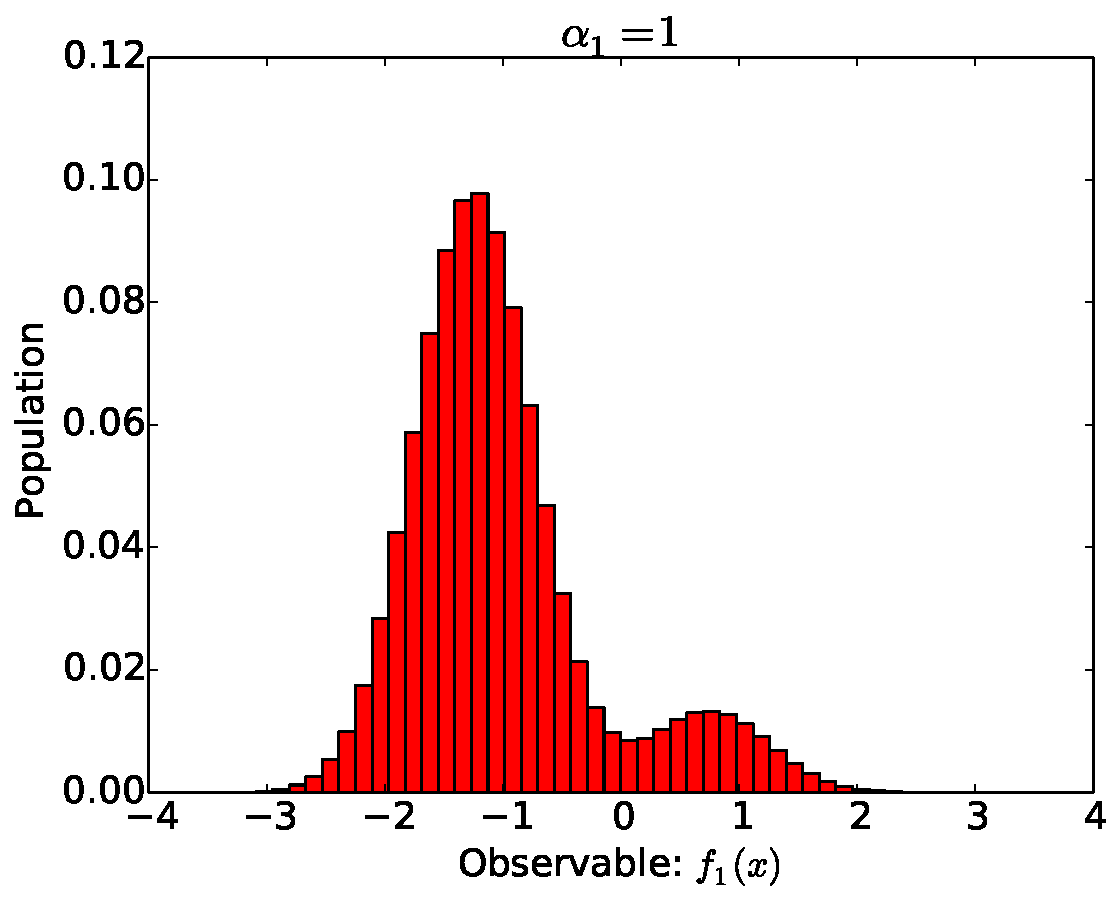
\includegraphics[width=5.0cm]{figures/model_hist1.pdf}
}

\subfigure[]{
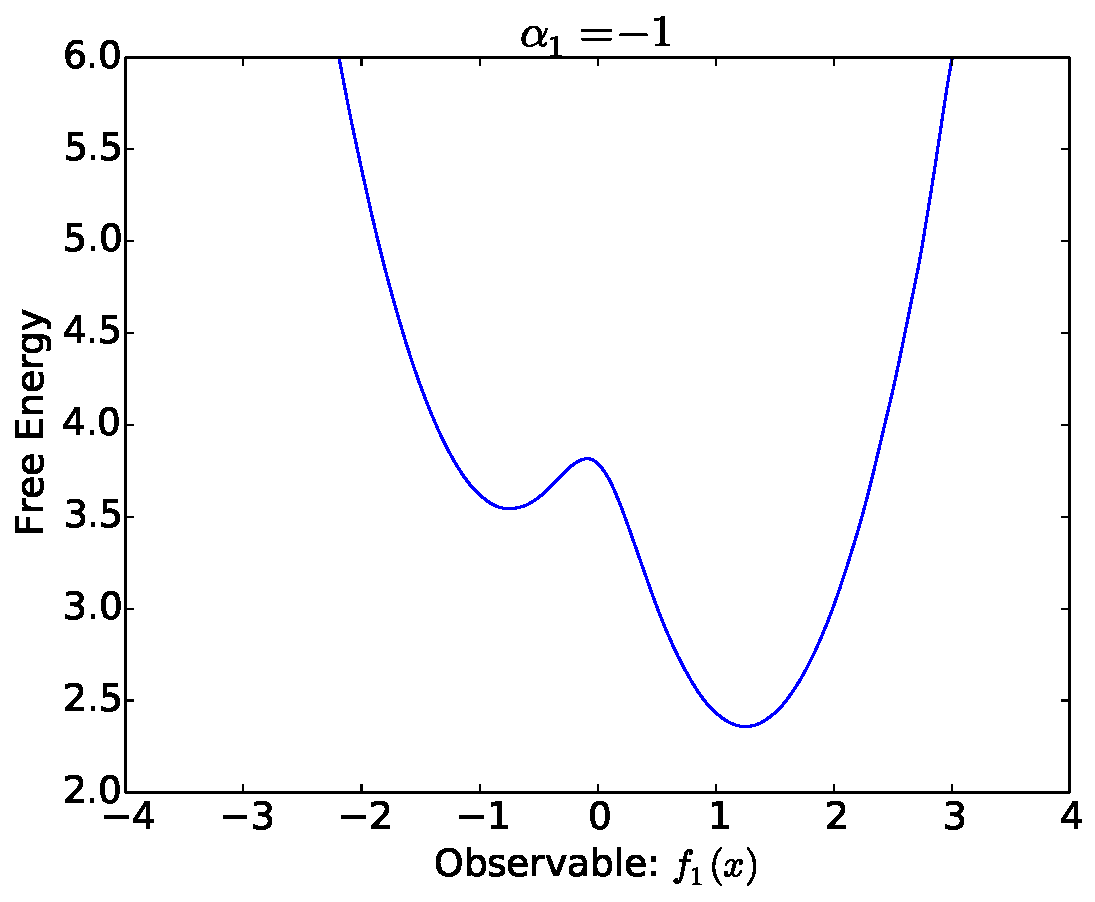
\includegraphics[width=5.0cm]{figures/model_landscape-1.pdf}
}
\subfigure[]{
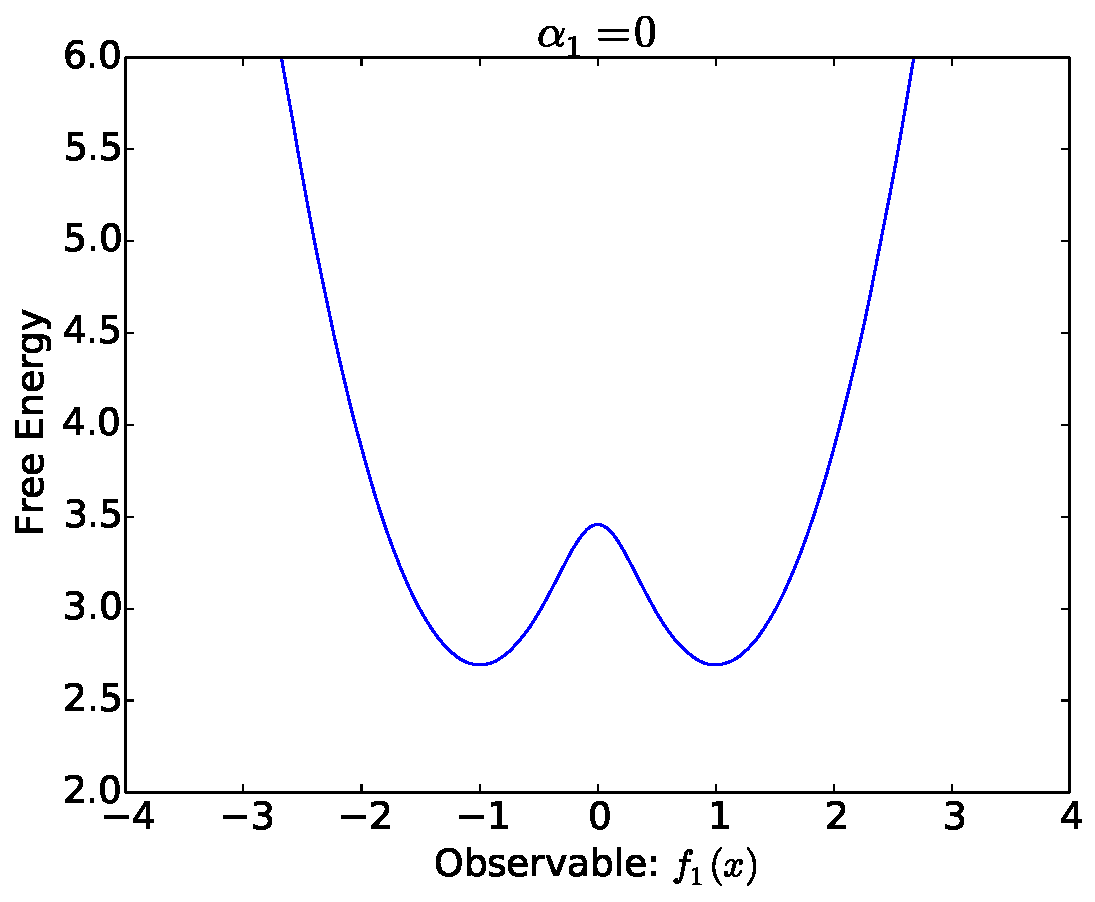
\includegraphics[width=5.0cm]{figures/model_landscape0.pdf}
}
\subfigure[]{
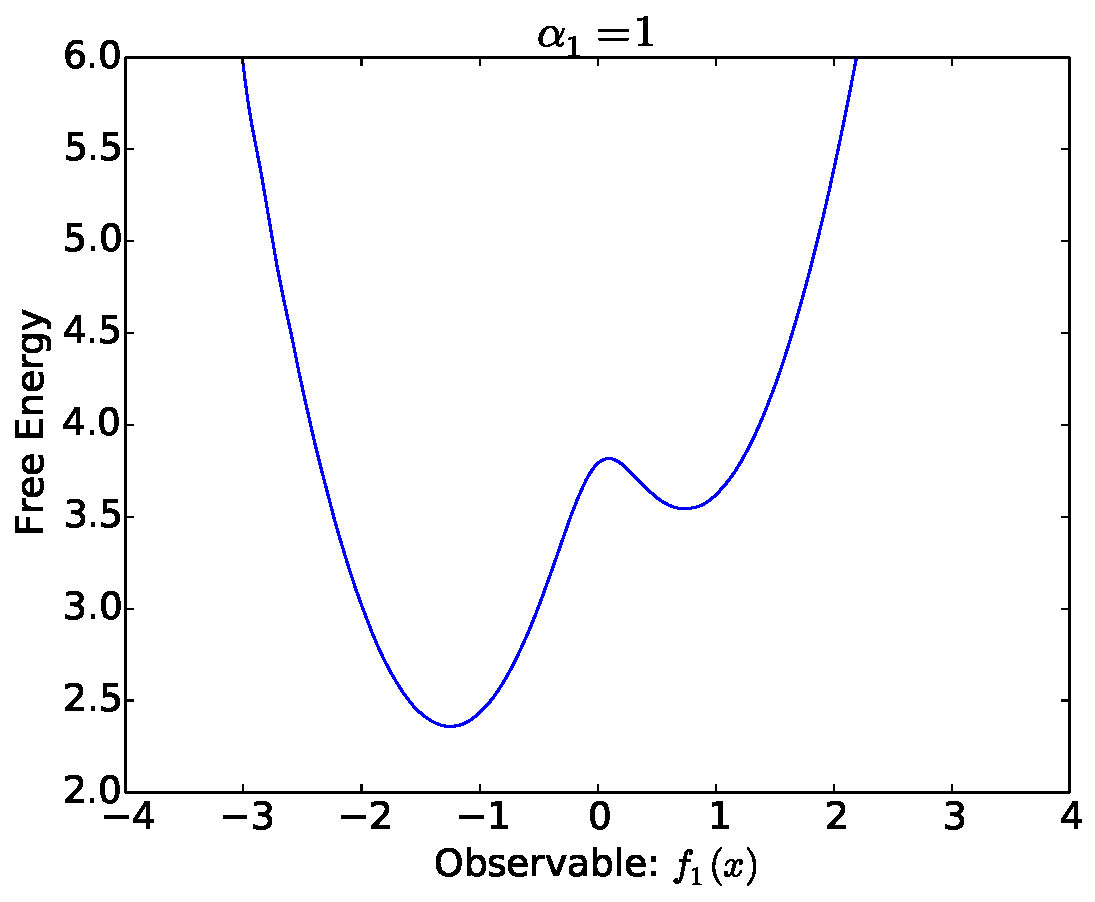
\includegraphics[width=5.0cm]{figures/model_landscape1.pdf}
}

\caption{
(a, b, c): Raw ($\alpha_1 = 0$) and reweighted (e.g. tilted) histograms of a one dimensional observable.  (d, e, f): The same, but plotted as free energies (e.g. $-kT \log(p)$).  
}
\label{figure:Hist}
\end{figure}

With the equilibrium populations, we can calculate the equilibrium expectations of an arbitrary observable $h(x)$:

$$\langle h(x)\rangle _\alpha = \sum_j h(x_j) \pi_j(\alpha)$$

In the above bracket notation, $\langle h(x)\rangle _\alpha$ is the ensemble average of $h(x)$ in an ensemble that is perturbed by a biasing potential $\Delta U(x;\alpha)$.  At this point, the determination of the parameters $\alpha_i$ has not yet been discussed.  The key idea, however, is that the $\alpha$ reweighted ensemble $\langle \rangle _\alpha$ should recapitulate the experimental measurements:

$$\langle f_i(x)\rangle _\alpha \approx F_i$$

Forcing this to be an exact equality recovers previous results \cite{chodera2012} that can be derived from maximum entropy considerations (Appx. S1); here, however, we take into account the experimental uncertainties associated with each $F_i$.  

\subsection*{Determining $\alpha$}

We now derive a Bayesian framework for determining the coefficients $\alpha$ used in the biasing potential.  An alternative derivation using the Crooks hyperensemble formalism \cite{crooks2007beyond} is given in Appx. S1.  BELT assumes that, given the correct choice of $\alpha$, the predicted observables $f_i(x)$ provide unbiased (but noisy) predictions of the measurements $F_i$.  This assumption is codified by the following conditional probability:

$$P(F_i | \alpha) \sim N(\langle f_i(x)\rangle _\alpha, \sigma_i^2)$$

For the current work, we model $\sigma_i$ as the uncertainty associated with predicting chemical shifts and scalar couplings from structures; this error is quantified by the RMS uncertainty estimated during the parameterization of chemical shift and scalar coupling models.  Using Bayes' Theorem, we can calculate the posterior distribution of $\alpha$:

$$P(\alpha | F_1, ..., F_n) \propto P(F_1, ..., F_n | \alpha) P(\alpha)$$

Now we let $LP(\alpha)$ denote the log posterior of $\alpha$ and simplify, dropping terms that are independent of $\alpha$:

$$LP(\alpha) = \log[ P(\alpha|F_1, ..., F_n)] = -\sum_i^n \frac{1}{2\sigma_i^2}(\langle f_i(x)\rangle _\alpha - F_i)^2 + \log P(\alpha) + constant$$

Note the simple form of the log posterior.  The first term (i.e. the log likelihood) measures the $\chi^2$ agreement between the reweighted ensemble and measurements.  The second term is the log of the prior distribution on $\alpha$.  

In the present work, we evaluate three different choices of prior (Appx. S4), finding similar results for each.  The first is the maximum entropy (maxent) prior, which penalizes ensembles as they deviate from the raw simulation results:

$$\log P(\alpha) = -\lambda \sum_j^m \pi_j(\alpha) \log \frac{\pi_j(\alpha)}{\pi_j^0}$$

In the previous expression, $\pi_j^0$ refers to the populations of an unweighted ensemble, which are typically $\frac{1}{m}$, while $\lambda$ is a hyperparameter that controls the strength of the prior.  We also consider using a Dirichlet prior, which is functionally similar to the maxent prior (Appx. S4):

$$\log P(\alpha) = -\lambda \sum_j \pi_j^0 \log \frac{\pi_j^0}{\pi_j(\alpha)}$$

The third prior we consider is a multivariate normal prior, where  $\alpha \sim N(0, \Sigma)$.  The value of $\Sigma$ is given by $\Sigma_{ij} = \lambda Cov(f_i(x), f_j(x))$, as derived in Appx. S4.

Each of these priors can be used to achieve regularization, which is a powerful technique to reduce overfitting \cite{friedman2001elements}.  Large values of $\lambda$ favor the raw simulation results (i.e. uniform conformational populations): $\pi_j \approx \pi_j^0 = \frac{1}{m}$.  The value of $\lambda$ can be chosen via cross-validation or other methods (see Appx. S5).  When using the maxent prior in the limit of $\lambda \rightarrow \infty$ and $\sigma \rightarrow 0$, BELT recovers the hyperensemble picture of nonequilibrium statistical mechanics as developed \cite{crooks2007beyond} by Crooks (See Appx. S1).  The Dirichlet and Normal priors do not share the same connection to the Crooks hyperensemble formalism; however, for normally distributed observables, all three priors will give identical results \cite{relative_entropy_wiki}.  

\subsection*{MCMC Sampling of Structural Ensembles}

As noted above, because ensemble inference often presents many plausible solutions  \cite{fisher2010, rieping2005}, we avoid statistical methods that return a single solution (e.g. maximum likelihood or maximum entropy).  We therefore use Markov chain Monte Carlo (MCMC), as implemented in PyMC  \cite{patil2010pymc}, to sample the distribution of structural ensembles consistent with experiment.  The result is an ensemble of ensembles--a statistical ensemble of conformational ensembles.  Averaging all MCMC samples provides posterior mean  estimates of arbitrary structural features or experimental observables.  Similarly, examining the MCMC variances provides statistical uncertainties of equilibrium or structural features.  A Bayesian bootstrapping procedure  \cite{rubin1981} can also be used to model the statistical uncertainty of the MD simulations (see Appx. S6).

\section*{Methods}

\subsection*{Molecular Dynamics Simulations}

Trialanine was simulated in the ff96 \cite{kollman1996}, ff99 \cite{wang2000}, ff99sbnmr-ildn \cite{li2010, Lindorff-Larsen2010}, CHARMM27 \cite{mackerell2004extending,bjelkmar2010implementation}, and OPLS-AA \cite{kaminski2001evaluation} force fields, as previously reported  \cite{beauchamp2012protein}.  Simulations were performed using Gromacs 4.5  \cite{hess2008} and run at constant temperature (300 K) and pressure (1.01 atm).  Each simulation was at least 225 ns long.  Conformations were stored every 1 ps.  

\subsection*{Chemical Shifts and Scalar Couplings}

All NMR measurements in this work refer to experiments  \cite{Graf2007} probing the central residue of trialanine.  Note that the experimental data was measured at pH 2, near the pKa of the carboxylate moiety of the C terminus.  This indicates that the true ensemble likely requires a constant pH simulation, rather than a fixed protonation state.  Because such simulations are challenging with current force fields and simulation packages, we simulated the trialanine construct with charged termini--where the the force fields have been best calibrated and tested.  We therefore focus our analysis on the central alanine residue, which should be most robust to pH dependent effects.  Both pH differences and force field inaccuracies will lead to systematic differences  between simulation and experiment; indeed, we assess whether BELT robustly corrects these deviations.  

Chemical shifts ($H$, $H^\alpha$, $C^\alpha$, $C^\beta$) for each frame were calculated using a weighted average of ShiftX2 \cite{han2011shiftx2}, SPARTA+  \cite{Shen2010}, and PPM \cite{li2012ppm} predictions; uncertainties for each model were estimated using their reported RMS prediction errors.  Overall uncertainties were estimated as $\sqrt{\sum w_i \sigma_i^2}$, where $w_i \propto \frac{1}{\sigma_i^2}$ is the weight ($\sum_i w_i = 1$) of each chemical shift model and $\sigma_i$ is the uncertainty of each chemical shift model.  The J couplings were calculated using the following Karplus relations: $^3J(H^N C')$  \cite{vogeli2007limits}, $^3J(H^N H^\alpha)$  \cite{vogeli2007limits}, $^2J(N C^\alpha)$  \cite{Graf2007}, $^3J(H^\alpha C')$  \cite{Schmidt1999}, $^1J(N C^\alpha)$  \cite{Graf2007}, $^3J(H^N C^\beta)$  \cite{vogeli2007limits}.  J coupling uncertainties were approximated as the RMS errors reported when fitting the Karplus coefficients.  

We have divided the available experimental measurements into training and test sets, with the training set consisting of the $^3J(H^N C')$,  $^2J(N C^\alpha)$, and $^3J(H^N C^\beta)$ scalar couplings and the $C^\alpha$, $H^N$, and $C^\beta$ chemical shifts.  The test set consists of $^3J(H^N H^\alpha)$, $^3J(H^\alpha C')$, $^1J(N C^\alpha)$, and the $H^\alpha$ chemical shift.  The division into training and test sets serves three purposes.  First, it provides a test of overfitting.  Second, it allows us to reduce the computational cost of BELT calculations.  Third, it allows us to train on data that are approximately uncorrelated; BELT is best suited for working with uncorrelated data.  Additional suggestions for data curation are provided in Discussion.  

\subsection*{BELT}

All BELT calculations were performed using the FitEnsemble package (\url{https://github.com/kyleabeauchamp/FitEnsemble}).  The online FitEnsemble tutorial demonstrates the use of BELT with a single experimental measurement ($^3J(H^N H^\alpha)$).  Source code for calculations in this work will be made available at \url{https://github.com/kyleabeauchamp/EnsemblePaper}.  

Regularization strength was determined via cross validation on the simulation data, as described in Appx. S5; this form of cross validation reduces errors due to finite sampling of equilibrium properties.  For each model, we used PyMC to sample at least 5,000,000 values of $\alpha$; sampled values of $\alpha$ were thinned 100-fold to reduce correlation.  The first 5,000 samples (before thinning) were discarded as burn-in.  Convergence of MCMC sampling was assessed by visual examination of MCMC traces; a well-sampled and thinned trace will appear to be white noise, without correlation between one sample and the next.  MCMC traces are shown in Fig. S2 and discussed in Appx. S7.  To incorporate simulation uncertainty, we used Bayesian Bootstrapping (Appx. S6).  Two Bayesian bootstrap replicates were performed.  

\section*{Results}

Short peptides provide crucial tests for evaluating and optimizing molecular dynamics force fields  \cite{Graf2007,beauchamp2012protein, nerenberg2011, best2008, Grdadolnik2011}.  Such peptides offer a window into the intrinsic conformational propensities of amino acids, free from the secondary structure bias found in statistical surveys of protein structures  \cite{Jha2005}.  Here, we use BELT to infer the conformational populations of trialanine from chemical shift and scalar coupling measurements  \cite{Graf2007}.  


\subsection*{Conformational Propensities of Trialanine Simulations}

Trialanine was simulated (see Methods) in five different force fields; these simulations are summarized here.  The chosen force fields show considerable variation in their predicted conformational propensities.  The ff96 force field shows a bias towards $\beta$ conformations (population: 51\%) (Fig. \ref{figure:ALA3}b, red).  On the other hand, ff99 strongly favors helical conformations, with a predicted $\alpha$ population of 80\% (Fig. \ref{figure:ALA3}c, red).  The $PP_{II}$ state, known to be the dominant state in solution \cite{Grdadolnik2011, Graf2007, Avbelj2006}, is the dominant simulated state only in the ff99sbnmr-ildn force field (Fig. \ref{figure:ALA3}a, red).  Low $PP_{II}$ populations and inconsistency between force fields have been previously noted \cite{Graf2007, beauchamp2012protein, nerenberg2011, best2008}.  

\subsection*{Agreement with NMR Measurements: MD and BELT Ensembles}

Given the differences in conformational propensities, one might expect varying degrees of agreement with the available experimental measurements.  This is indeed the case; four out of five force fields show large values of the reduced $\chi^2$ (e.g. $\frac{1}{n} \chi^2$) (Fig. \ref{figure:ChiSquared}a, red).  Because of this considerable error, we therefore examined BELT ensembles trained on six NMR measurements.  As expected, the BELT ensembles accurately recapitulate these six measurements (Fig. \ref{figure:ChiSquared}a).  In a more incisive test, the BELT ensembles accurately predict four measurements that were not used to fit the models.   (Fig. \ref{figure:ChiSquared}b).  A table of predicted and observed NMR measurements is given in Tables \ref{table:Predictions}, S1, and S2.  

\subsection*{Converged Conformational Propensities Observed in BELT Ensembles}

Although the raw MD simulations predicted quite different conformational propensities, BELT reweighting gives five ensembles with conformational populations that agree to within statistical uncertainty (Fig. \ref{figure:ALA3}).  In general, we find ($PP_{II}$, $\beta$, $\alpha$) populations of (67 $\pm$ 9\%, 23$\pm$ 6\%, 10$\pm$ 8\%); here the mean and uncertainty are approximated as the mean and standard deviation across all force fields and priors.  Quantitative predictions and uncertainties are given in Tables S3-S6.  

\subsection*{Effect of Prior}

In addition to convergence between models constructed from different force fields, one can also assess the convergence between BELT models built using different priors on the parameters $\alpha$.  In general, different priors give similar results with small quantitative differences (Figs. \ref{figure:ALA3} and \ref{figure:ChiSquared}).  Building BELT models with different priors could therefore be useful for bracketing uncertainties in situations with limited simulation data.  

\subsection*{The Resolution Limit of Trialanine BELT Ensembles}

Despite the near-quantitative agreement in $\alpha$, $\beta$, and $PP_{II}$ populations (Fig. \ref{figure:ALA3}) and overall Ramachandran features (Fig. \ref{figure:Rama}), the fine structure of the Ramachandran plots differs between the five models.  Because all five BELT ensembles show excellent agreement with experiment (Fig. \ref{figure:ChiSquared}), we conclude that six chemical shifts and scalar couplings are insufficiently informative to resolve (and falsify) subtle force field differences.  The most obvious such difference is the width, shape, and orientation of the $PP_{II}$ basin.  Most strikingly, ff96 and OPLS-AA have $PP_{II}$ basins that are vertically oriented, while ff99, ff99sbnmr-ildn, and CHARMM27 show diagonally oriented $PP_{II}$ basins.  Two different effects contribute to this resolution limit: the information content in the experimental measurement and the uncertainty in predictors of experimental observables.


\begin{figure}
\subfigure[]{
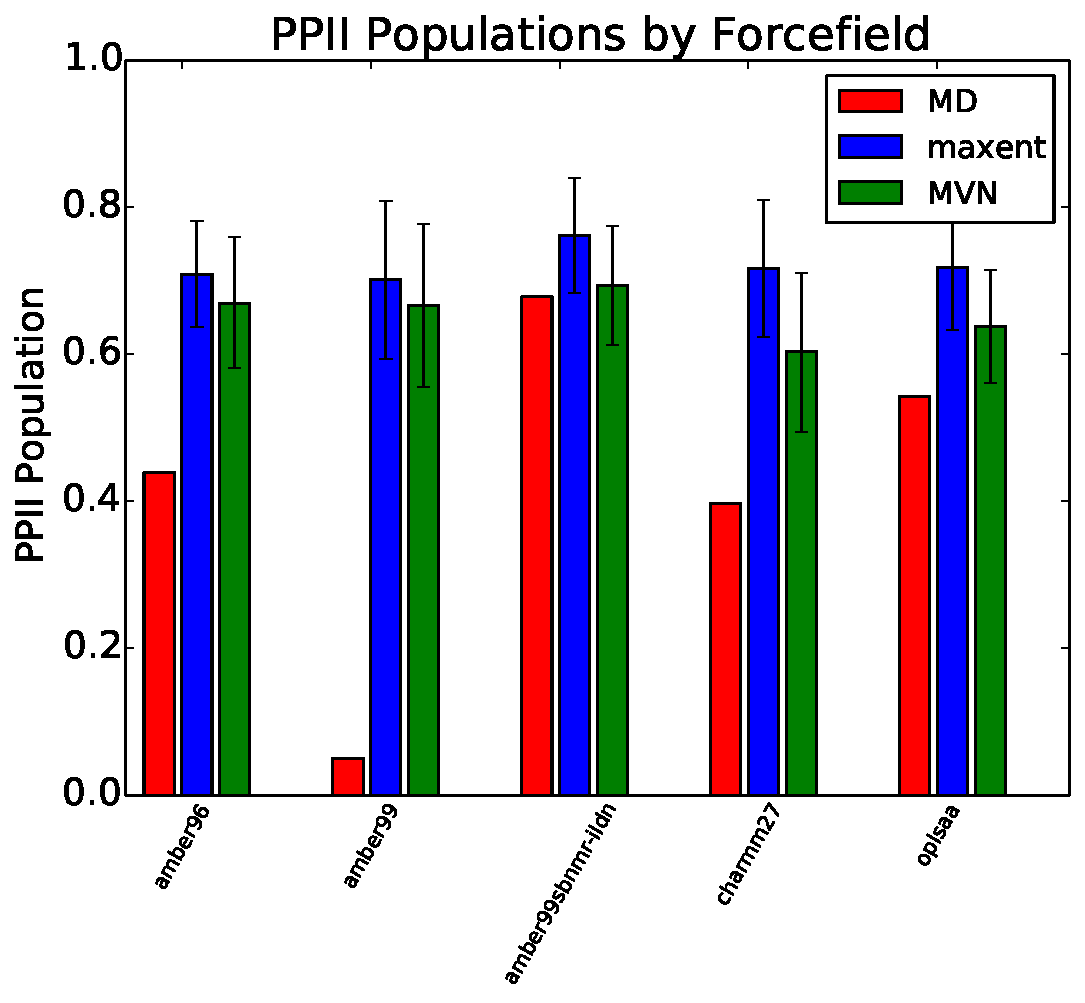
\includegraphics[width=7.5cm]{figures/state_0_by_forcefield_priors.pdf}
}

\subfigure[]{
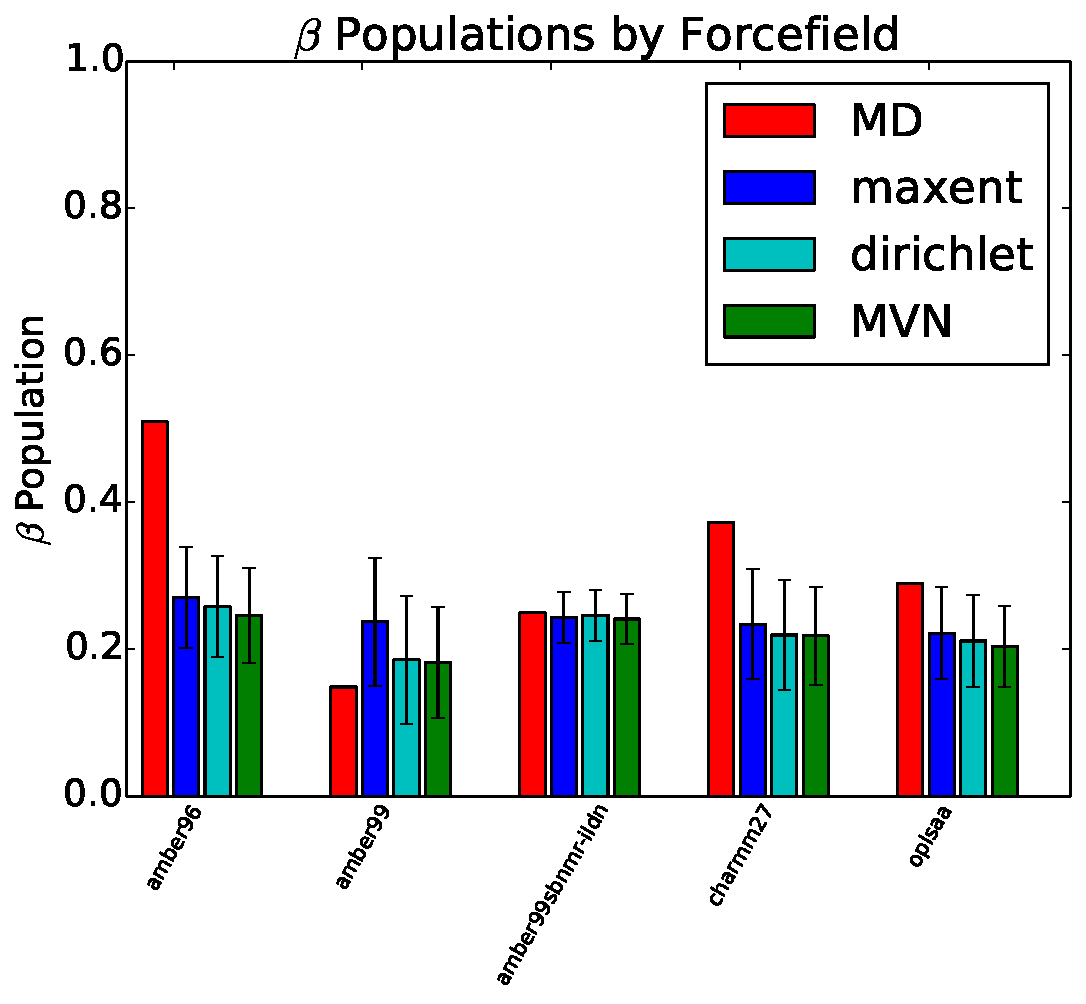
\includegraphics[width=7.5cm]{figures/state_1_by_forcefield_priors.pdf}
}
\subfigure[]{
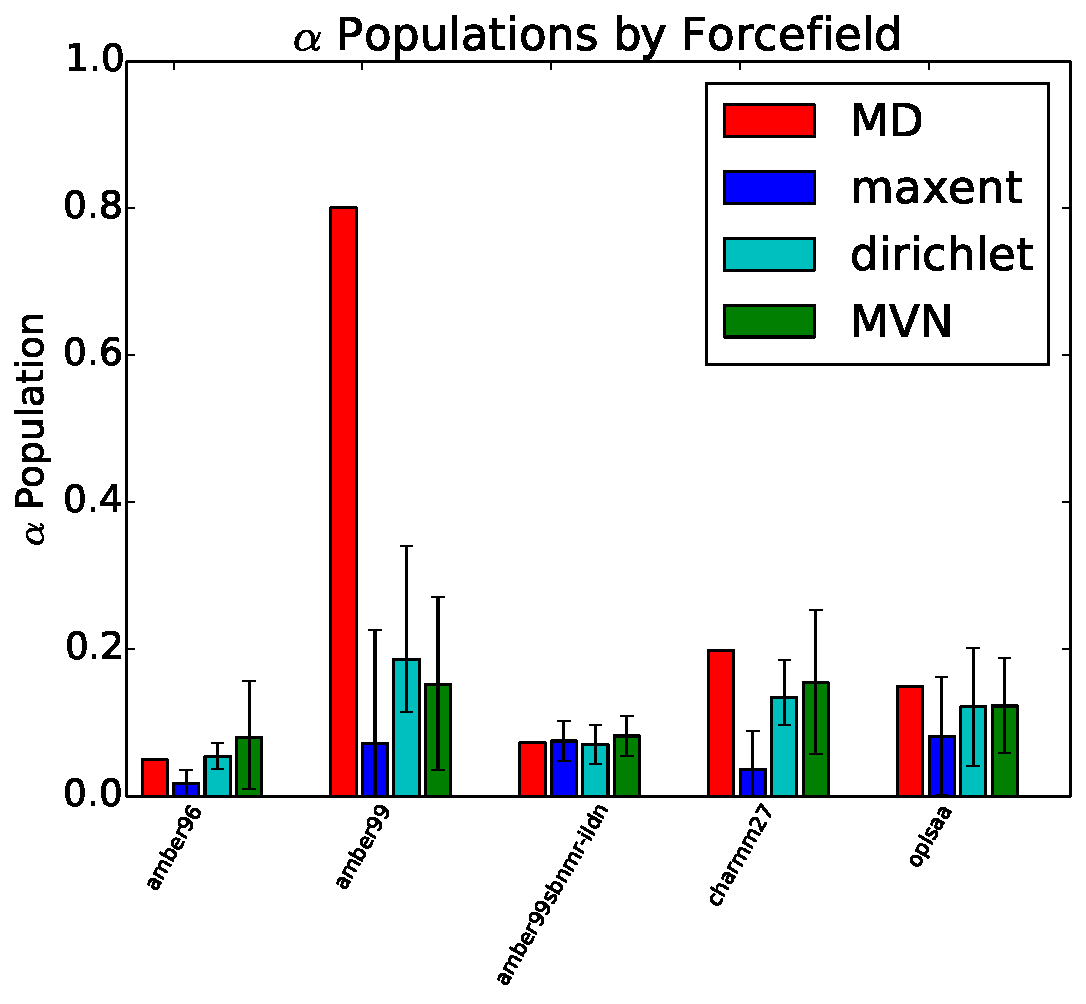
\includegraphics[width=7.5cm]{figures/state_2_by_forcefield_priors.pdf}
}
\caption{
MD and BELT (maxent, Dirichlet, and MVN priors) conformational propensities (for central alanine residue) in each force field.  
}
\label{figure:ALA3}
\end{figure}


\begin{figure}
\subfigure[]{
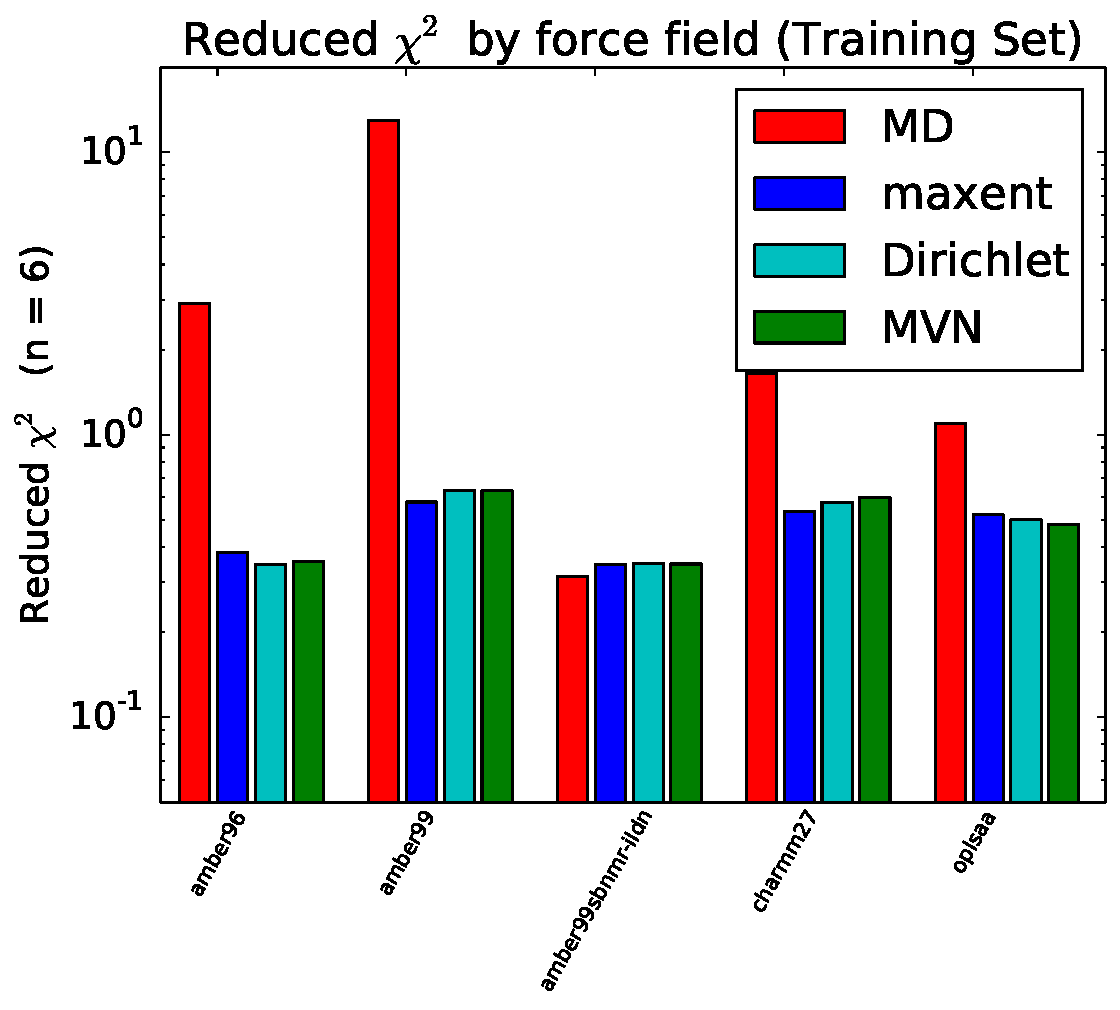
\includegraphics[width=7.5cm]{figures/chi2_train_priors.pdf}
}
\subfigure[]{
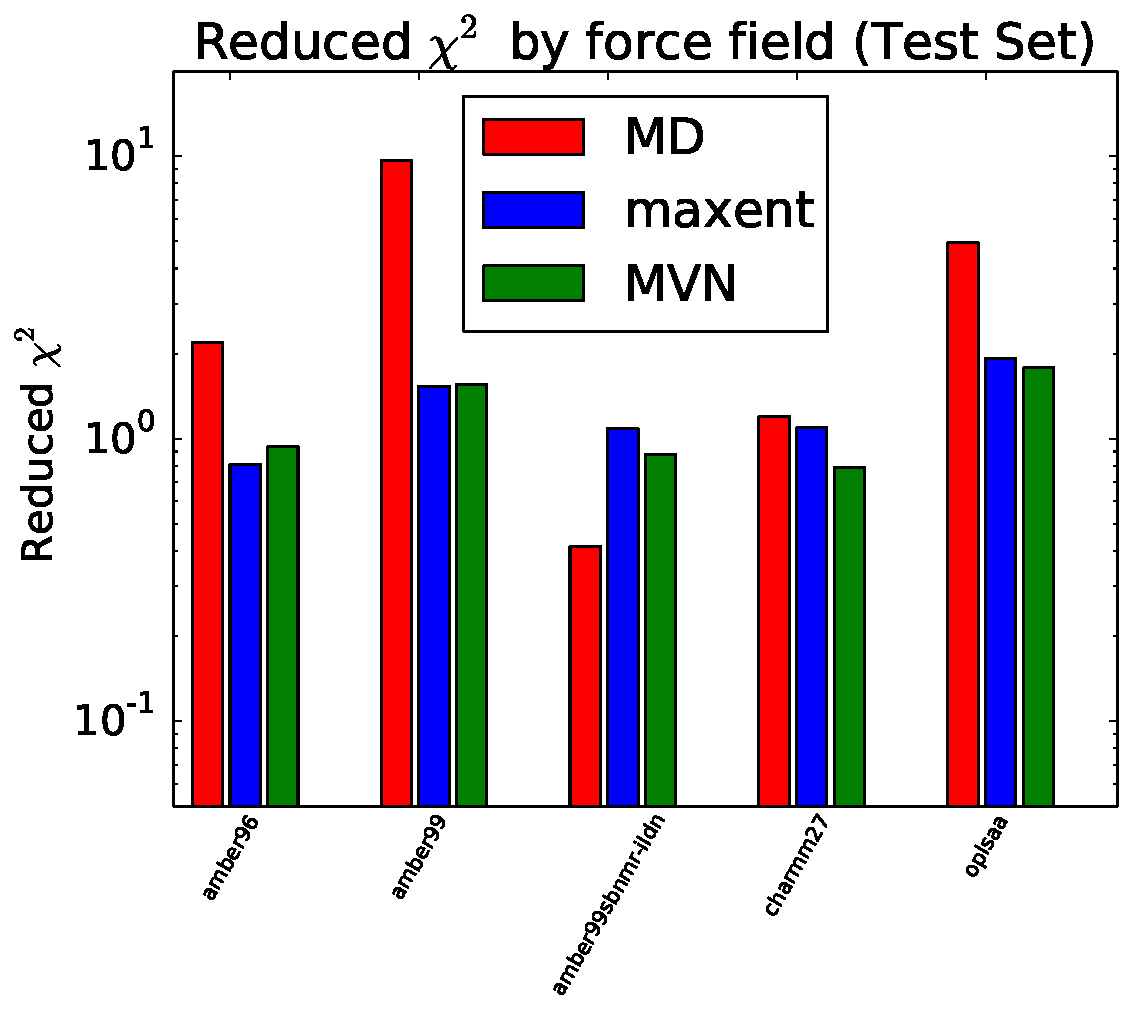
\includegraphics[width=7.5cm]{figures/chi2_test_priors.pdf}
}
\caption{
The reduced $\chi^2$ error (e.g. $\frac{\chi^2}{n}$) for MD and BELT (maxent, Dirichlet, and MVN priors) models.  The BELT reduced $\chi^2$ is estimated as the mean reduced $\chi^2$ over all MCMC samples.  (a).  Calculated using the six measurements used to fit the BELT model.  (b).  Calculated using four measurements not used to fit the BELT model.  See Methods for the definition of training and test sets.  Note that the training and test sets are not fully independent because all measurements probe the $(\phi, \psi)$ backbone torsions.
}
\label{figure:ChiSquared}
\end{figure}


\begin{figure}
\subfigure[]{
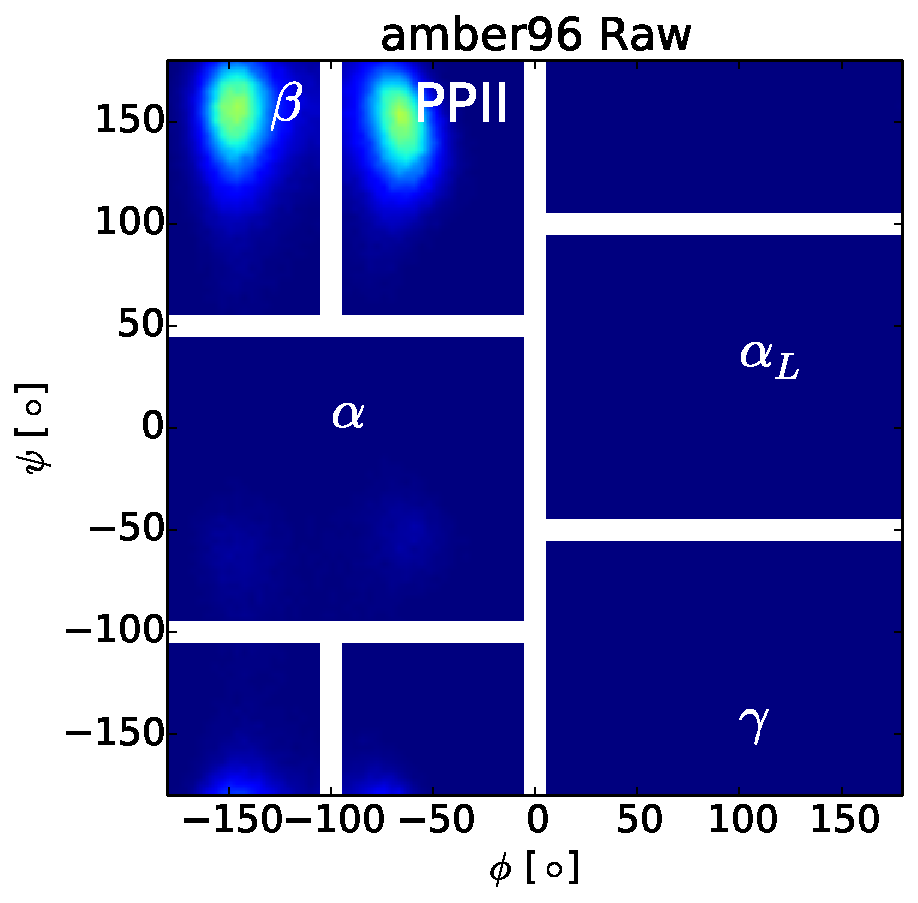
\includegraphics[width=3.05cm]{figures/ALA3_rama_amber96_raw.pdf}
}
\subfigure[]{
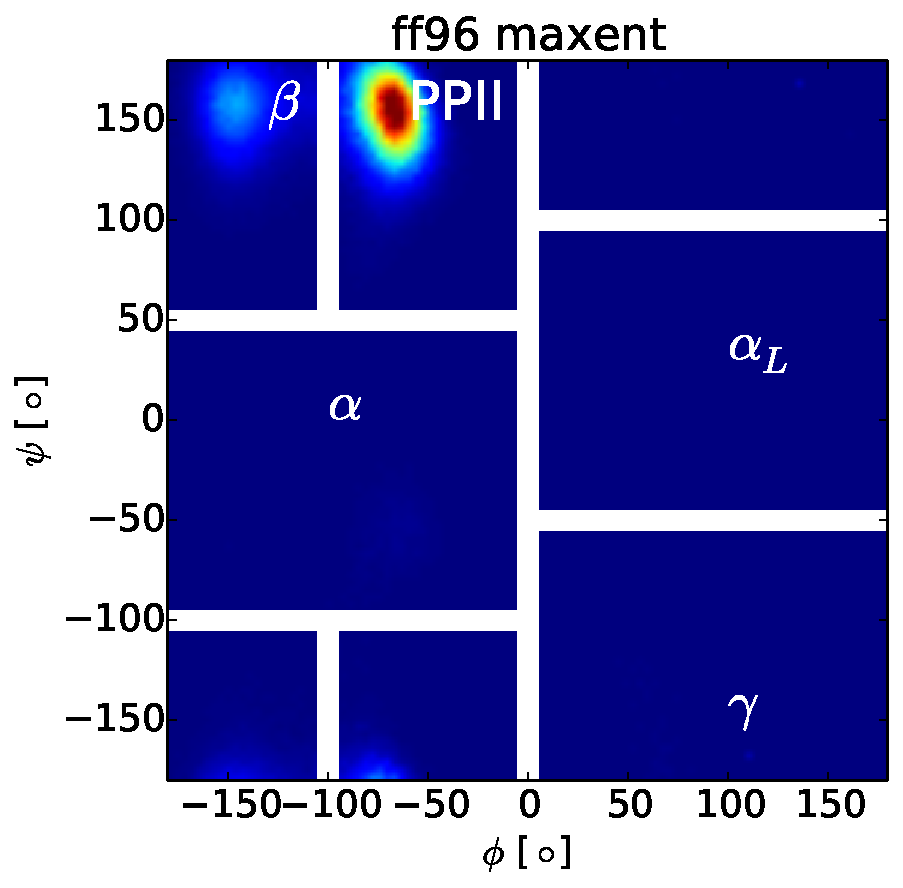
\includegraphics[width=3.05cm]{figures/ALA3_rama_amber96_maxent_belt.pdf}
}

\subfigure[]{
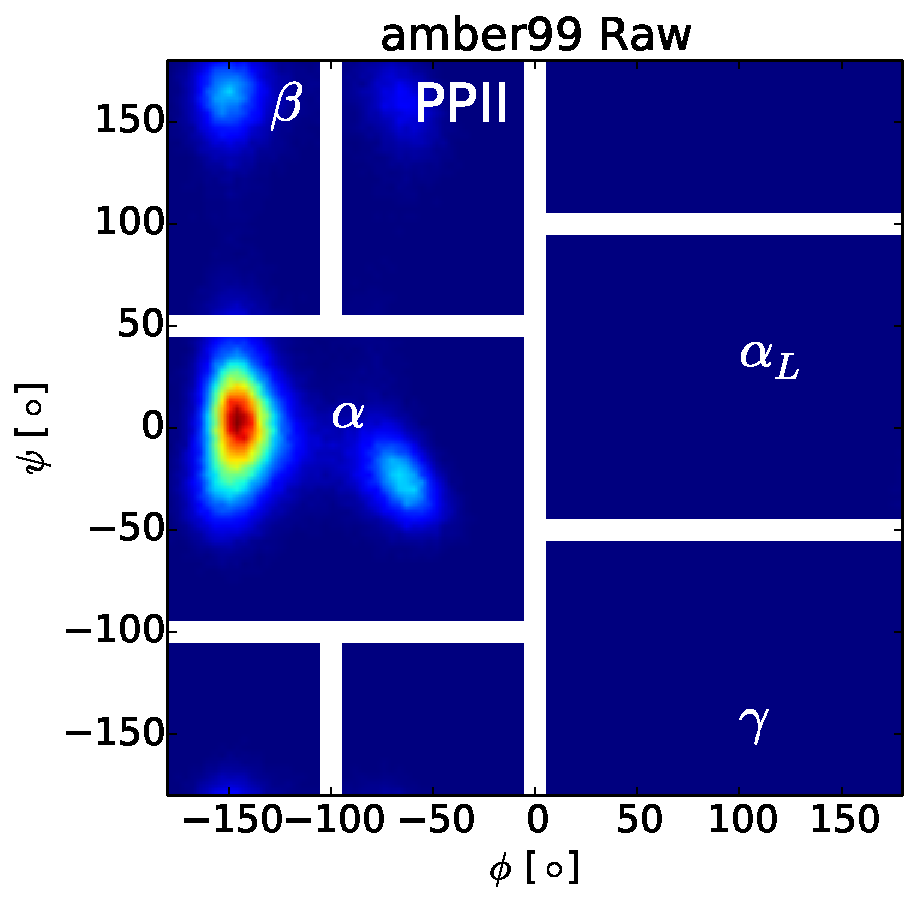
\includegraphics[width=3.05cm]{figures/ALA3_rama_amber99_raw.pdf}
}
\subfigure[]{
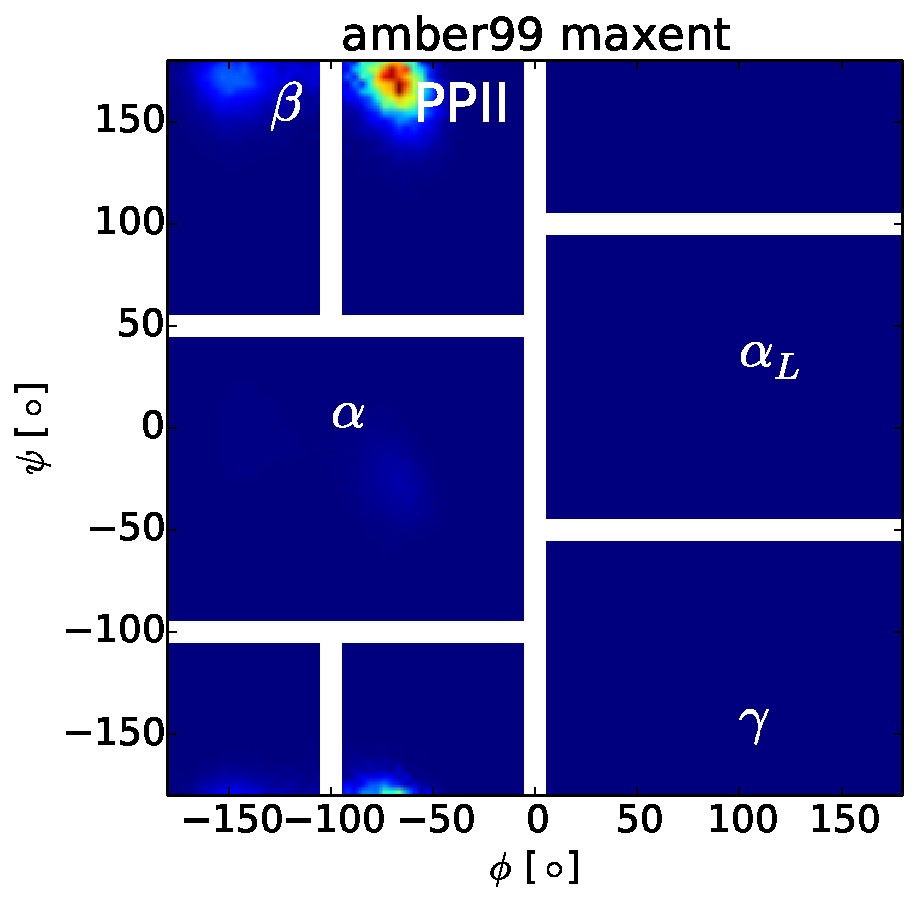
\includegraphics[width=3.05cm]{figures/ALA3_rama_amber99_maxent_belt.pdf}
}

\subfigure[]{
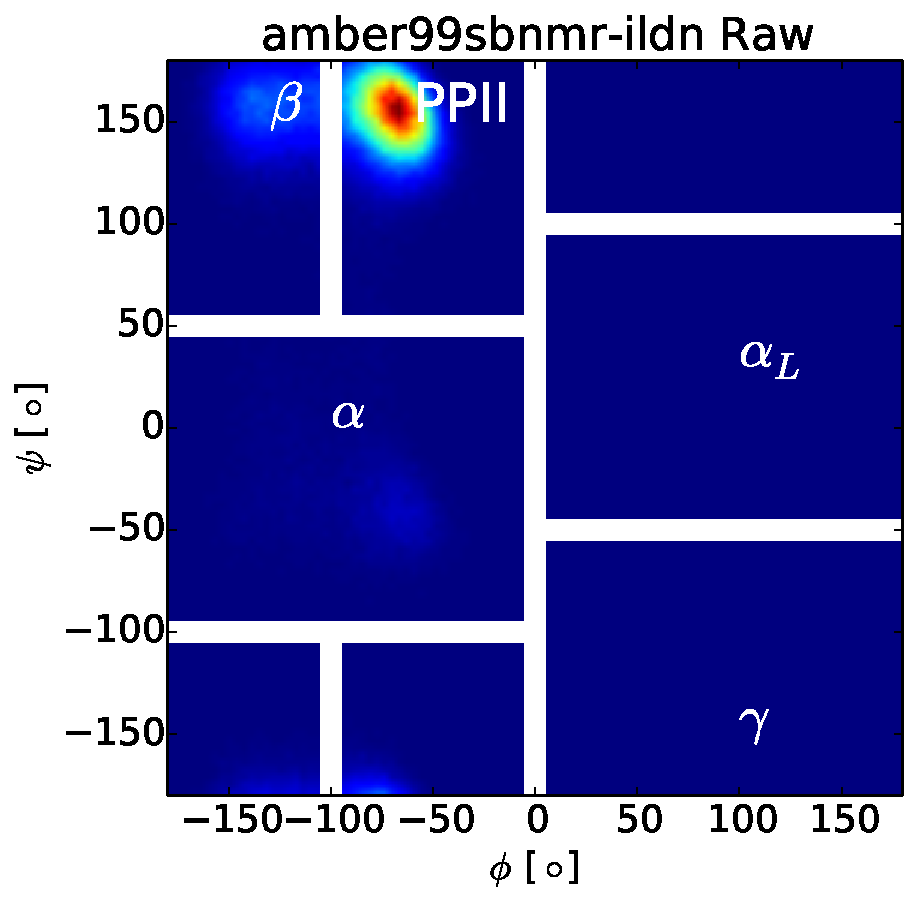
\includegraphics[width=3.05cm]{figures/ALA3_rama_amber99sbnmr-ildn_raw.pdf}
}
\subfigure[]{
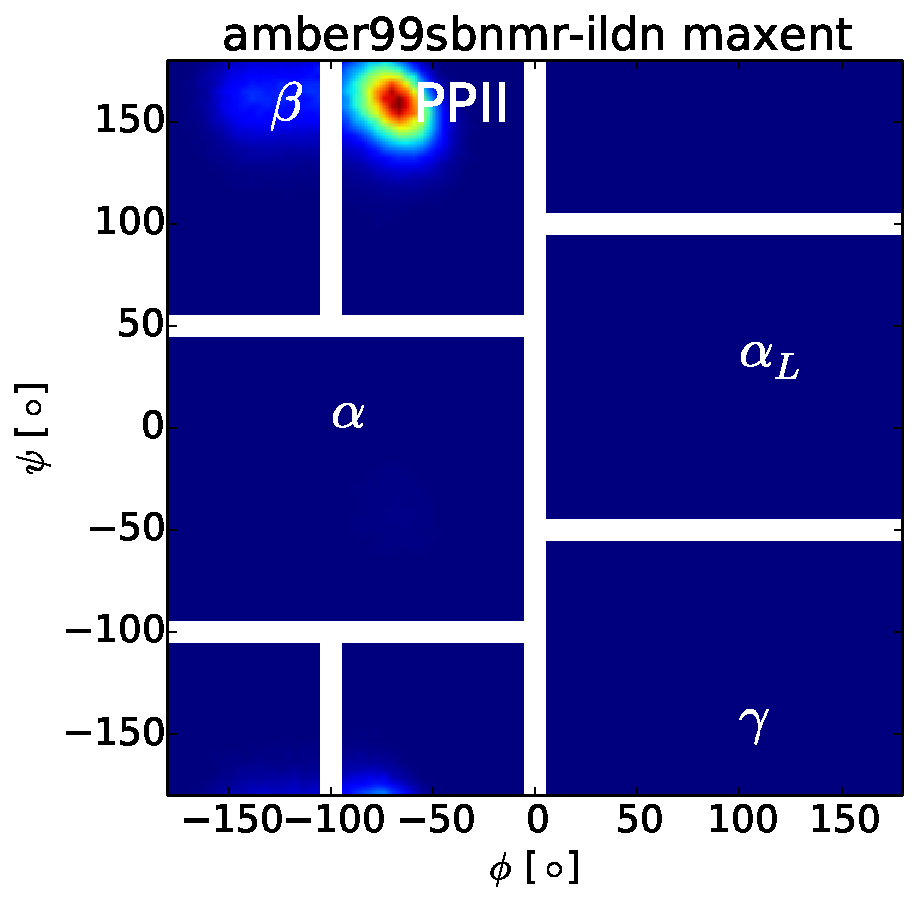
\includegraphics[width=3.05cm]{figures/ALA3_rama_amber99sbnmr-ildn_maxent_belt.pdf}
}

\subfigure[]{
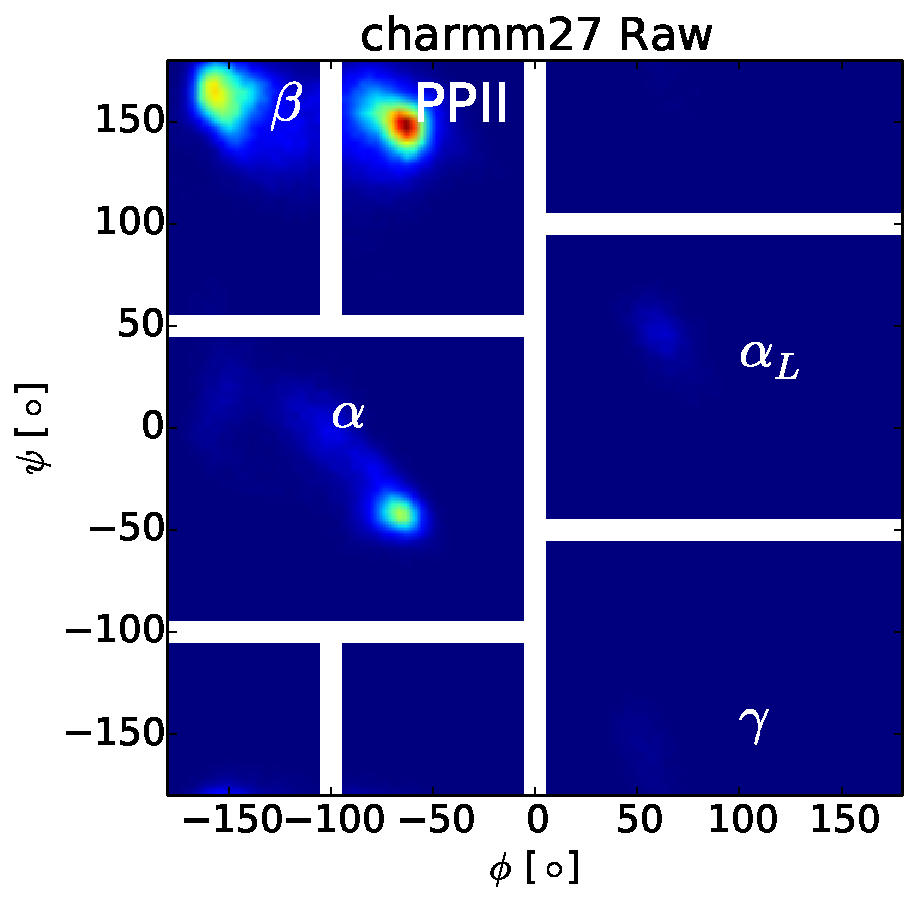
\includegraphics[width=3.05cm]{figures/ALA3_rama_charmm27_raw.pdf}
}
\subfigure[]{
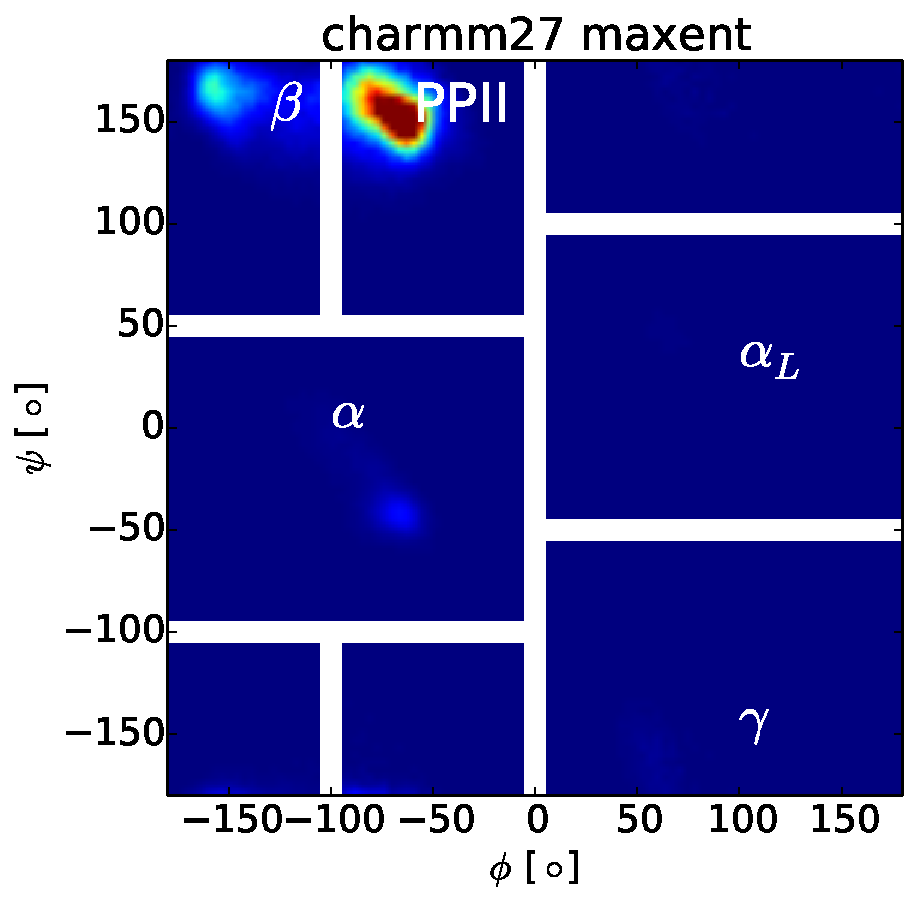
\includegraphics[width=3.05cm]{figures/ALA3_rama_charmm27_maxent_belt.pdf}
}

\subfigure[]{
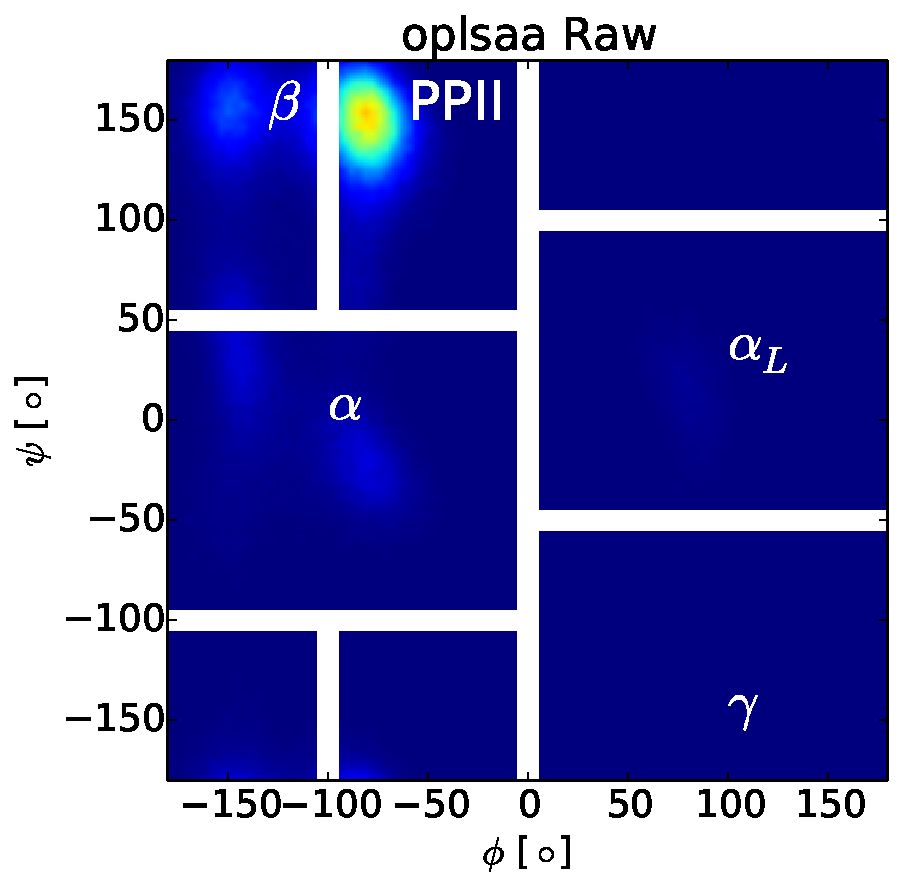
\includegraphics[width=3.05cm]{figures/ALA3_rama_oplsaa_raw.pdf}
}
\subfigure[]{
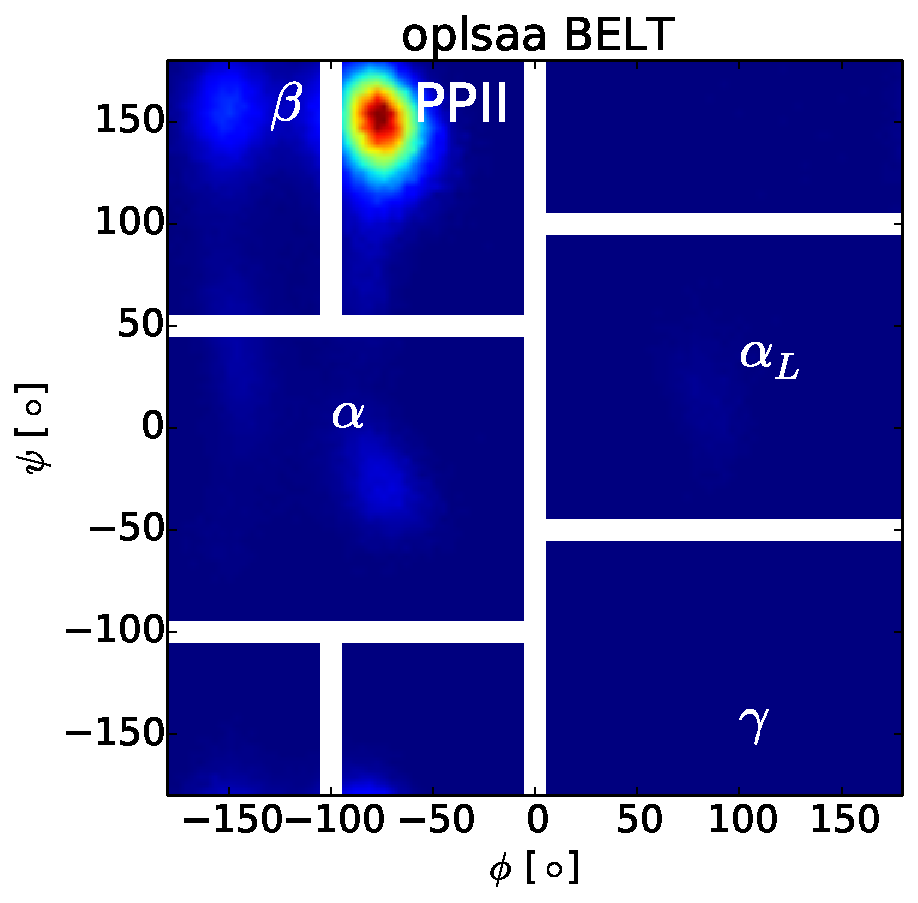
\includegraphics[width=3.05cm]{figures/ALA3_rama_oplsaa_maxent_belt.pdf}
}

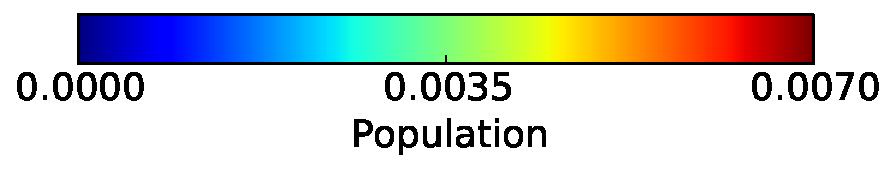
\includegraphics[width=3.05cm]{figures/ALA3_rama_colorbar.pdf}


\caption{
Ramachandran plots of MD and BELT (maxent prior) ensembles for each force field; additional priors are shown in Fig. S1.  The jagged appearance of the ff99 BELT model is due to limited sampling of PPII configurations in that forcefield.  
}
\label{figure:Rama}
\end{figure}

\section*{Discussion}

\subsection*{Structural Ensemble Biology}

Why model structural ensembles, rather than just structures?  At least three compelling reasons favor ensembles.  First, biological molecules are multi-state machines that fold, unfold, bind ligands, aggregate, and change conformation.  Biology is controlled by the relative populations of these states.  Ensembles capture aspects of these phenomena by encoding equilibrium populations with structures.  A second argument for ensemble modeling is fidelity to experiment.  Most solution experiments measure ensemble average equilibrium properties--chemical shifts, scalar couplings, NOEs, SAXS, and FRET can often be approximated as equilibrium properties.  A truly quantitative connection to these measurements requires modeling the equilibrium ensemble.  Finally, recent advances in atomistic simulation  \cite{hess2008, pronk2013gromacs, eastman2012openmm, eastman2010openmm}, special-purpose hardware  \cite{Shaw2008}, and distributed computing analysis  \cite{emma, msmb2} have enabled atomistic simulations to 
reach the millisecond timescale  \cite{voelz2010, bowman2011atomistic, shaw2010, Shaw2011}; the computational cost of ensemble modeling is quickly becoming manageable.

One might argue that structural ensembles are unnecessary because many proteins occupy a single state under physiological conditions.  For such proteins, it is probably safe to enforce single state behavior, as is done in current modeling approaches. However, we suggest that the number of states be inferred--not assumed.  

\subsection*{Comparison to Previous Ensemble Methods}

Most previous ensemble modeling efforts involve a protocol with three key ingredients: state decomposition, a $\chi^2$ objective function, and population inference on the clusters.  For example, this general recipe describes the approach used in previous analyses of homopeptides  \cite{Graf2007}, the EROS technique for SAXS modeling  \cite{rozycki2011saxs}, and the Bayesian Weighting (BW) formalism  \cite{fisher2010}.  Note that of these three techniques, only BW goes beyond returning a single best-fit ensemble and instead characterizes the posterior distribution via MCMC; below we therefore focus our attention on BW as it is most directly comparable to BELT in scope and purpose.

The primary disadvantage of previous techniques is the need for a state decomposition, which can be defined either by hand or by clustering.  Working with a given state decomposition can introduce two different errors, depending on the number  and quality of states.  In the limit of few states, clustering can overly coarsen the system of interest, preventing the model from reproducing multiple experimental observables.  At the other extreme, too many states leads to a large number of parameters to be estimated. This will lead to poor generalization performance and large errors when predicting experiments not used to train the model, as well as reliance on a subjective choice of how many states is appropriate.  One symptom of this regime is discontinuity in conformational populations. For example, imagine two nearby conformations at the boundary between two BW states--one conformation on each side of the boundary.  In BW, the populations of each conformation could fluctuate dramatically with the 
corresponding 
state populations.  In BELT, however, the two conformations will have nearly identical populations if the predicted observables vary smoothly.

BELT avoids arbitrary state decompositions by projecting simulations onto a basis defined by the predicted experimental observables.  The advantage of working in this basis are threefold. First, in BELT, one estimates a single parameter ($\alpha_i$) for each experimental observable.  If the number of experiments is small, as is often the case, the inference problem involves only a few parameters.  Second, the predicted observables are a natural basis for biophysical calculations, in that the predicted observables are the fundamental connection between simulation and experiment.  Working in this basis allows direct connection to experiment and often provides insight into the molecular interactions driving biophysical phenomena.  For example, the projection onto observables could be used to rationally infer force field parameters--essentially a Bayesian version of the ForceBalance method  \cite{wang2012, wang2013systematic}.  Third, in the limit of exact measurements, BELT reduces to a previous  \cite{
chodera2012} maximum entropy approach (see Appx. S1).  

We also point out some surprising differences between BELT and BW-like methods.  BW-like methods have the property that the in-state means of features are preserved, leading to an undesirable dependence on the choice of state decomposition.  More precisely, suppose that $\chi_s(x)$ is the indicator function of a conformational state $s$.  Then in-state averages of the form $<\chi_s(x)>^{-1} <h(x) \chi_s(x)>$ do not depend on the reweighted populations.  BELT, however, does not preserve the in-state averages; in fact, this property is the direct result of BELT's connection to maximum entropy modeling (see Appx. S1 and ref.  \cite{chodera2012}).  The effect of this property is that the peaks of reweighted histograms are slightly shifted relative to the raw MD results, as observed in Fig. \ref{figure:Hist}.   

\section*{Comparison to a Previous Trialanine Study}

Our results are in qualitative, but not quantitative, agreement with a previous study of trialanine \cite{Graf2007}.  That study suggested a $PP_{II}$ population as high as $92 \pm 5\%$, somewhat higher than our $67 \pm 9 \%$ and with a twofold lower estimated uncertainty.  The difference can be attributed to three methodological differences.  First, the previous study used likelihood maximization to directly fit the ($PP_{II}$, $\beta$, and $\alpha$) populations from a three-state decomposition of their simulations.  The use of likelihood maximization may give misleading results when the likelihood surface is broad and shallowly peaked, as was found in the previous study.  However, this does not appear to be the primary cause of disagreement, as maximization of the BELT likelihood recovers populations within $\pm 5\%$ of the values obtained via MCMC sampling.  Second, the previous study assumed each scalar coupling to have an uncertainty of 1, while we approximate the uncertainties as the RMS errors 
determined when fitting the Karplus equations.  This weights the measurements differently and will lead to quantitative differences in estimated populations.  Different choices of Karplus coefficients also may lead to different predicted properties, as has been discussed elsewhere \cite{markwick2009structural}.    Finally, differences in state decomposition may cause slight differences in estimated conformational populations.  


\section*{Curating Data and Errors for BELT}

Because the BELT log likelihood weights errors quadratically, it is vital to use the highest quality experimental measurements, predictions, and error estimates.  We recommend that users manually inspect all measured and predicted observables before performing BELT analysis.  As discussed above, understanding the errors on different measurements affects the inferred ensemble properties.  We discuss another example we encountered in the current analysis.  

Scalar couplings predicted using parameterized Karplus relations will span a limited range that is determined by the Karplus coefficients.  In several cases, however, experimentally measured J couplings lie outside this range--meaning that even a perfect force field would be unable to recapitulate the experimental measurements.  Such measurements indicate limits in the transferability of simple Karplus prediction of scalar couplings; any such examples are best excluded from BELT analysis.  Improved  Karplus models for scalar couplings are clearly desirable.  

\section*{Limitations of BELT}

There are several limitations of the BELT method.  Most obvious is that BELT can only reweight existing simulations.  The force field used must be sufficiently accurate to sample experimentally-consistent conformations.  Achieving accurate predictions using poor force fields may require orders of magnitude more MD sampling.  The same increased sampling requirements apply as one attempts to fit many measurements simultaneously.  In the worst-case scenario, fitting $n$ measurements could require MD datasets whose size grows exponentially with $n$.  A second limitation in BELT is its computational cost.  In the present calculations, MCMC sampling for each model took approximately 24 hours.  These datasets included six measurements and approximately 250,000 conformations.  Because using additional conformations is computationally prohibitive, BELT ensembles are essentially limited to resolving states that have populations of at least $\frac{1}{250000}$.  A third limitation is the independent normal approximation 
used in BELT's error model (see Appx. S3).  More sophisticated error models may be possible, including the Bayesian formalisms from the Nilges group \cite{rieping2005, habeck2006, habeck2005bayesian}.  Another limitation is that BELT restricts modeling to ensembles whose log-populations can be represented by a linear combination of observables.  Finally, BELT is currently formulated for use with equilibrium measurements, meaning that the present framework cannot be used to predict kinetic properties.  

\section*{Conclusion}

Bayesian Energy Landscape Tilting allows the simultaneous characterization of structural and equilibrium properties.  Through its use of MCMC, BELT is robust to ambiguous experiments and provides rigorous uncertainty estimates, as illustrated here in the case of a simple tripeptide system.  BELT models constructed with a handful of NMR measurements correct significant force field bias and provide generalizable, force field independent trialanine ensembles.  The principled combination of simulation and experiment will enable robust, incisive predictions of the atomic-scale behavior of macromolecules--predictions that might not be achievable using either simulation or experiment alone.  


\section*{Acknowledgements}

We thank John Chodera, TJ Lane, Frank Cochran, Pehr Harbury, Xuesong Shi, and Dan Herschlag for helpful discussions.  

\clearpage

\begin{table}

\small

\begin{tabular}{lrrrrrrrrrrrr}
\toprule
   &  $F_i$ &  $\sigma_i$ &  \multicolumn{2}{c}{ff96}             &  \multicolumn{2}{c}{ff99}    &  \multicolumn{2}{c}{ff99sbnmr-ildn}   &  \multicolumn{2}{c}{CHARMM27}       &  \multicolumn{2}{c}{OPLS-AA}               \\
   &        &             &  MD   & BELT & MD   & BELT & MD   & BELT & MD   & BELT & MD   & BELT  \\
         &      &              &          &                 &          &                 &                    &                           &           &                  &         &                \\
$C^\alpha$           & 52.4 &          0.9 &     52.1 &            52.2 &     52.8 &            52.5 &               52.4 &                      52.4 &      52.5 &             52.4 &    52.2 &           52.2 \\
$C^\beta$           & 19.2 &          1.0 &     20.0 &            19.8 &     18.0 &            18.8 &               18.3 &                      18.4 &      18.2 &             18.6 &    19.6 &           19.6 \\
$H$            &  8.6 &          0.5 &      8.6 &             8.6 &      8.3 &             8.4 &                8.2 &                       8.2 &       8.3 &              8.3 &     8.6 &            8.6 \\
$H^\alpha$           &  4.4 &          0.2 &      4.6 &             4.6 &      4.6 &             4.6 &                4.5 &                       4.5 &       4.6 &              4.6 &     4.6 &            4.6 \\
$^1J(NC^\alpha)$      & 11.3 &          0.5 &     11.3 &            11.5 &     10.4 &            11.8 &               11.5 &                      11.5 &      11.2 &             11.7 &    11.1 &           11.3 \\
$^3J(H^\alpha C\prime)$ &  1.8 &          0.4 &      2.0 &             1.7 &      2.2 &             1.7 &                1.8 &                       1.8 &       2.0 &              1.8 &     2.2 &            2.0 \\
$^3J(H^NC^\beta)$     &  2.4 &          0.2 &      1.5 &             2.3 &      0.8 &             2.3 &                2.3 &                       2.3 &       1.8 &              2.3 &     1.9 &            2.2 \\
$^3J(H^NC\prime)$ &  1.1 &          0.3 &      1.5 &             1.2 &      1.8 &             1.2 &                1.0 &                       1.0 &       1.4 &              1.2 &     0.9 &            0.8 \\
$^3J(H^NH^\alpha)$     &  5.7 &          0.4 &      6.6 &             5.7 &      7.5 &             5.6 &                6.1 &                       6.0 &       6.3 &              5.7 &     7.0 &            6.5 \\
$^2J(NC^\alpha)$      &  8.4 &          0.5 &      8.5 &             8.6 &      6.4 &             8.5 &                8.5 &                       8.5 &       8.1 &              8.6 &     8.1 &            8.4 \\
$\chi^2$ (all)                           &    &            &      2.5 &             0.6 &     10.8 &             1.0 &                0.4 &                       0.4 &       1.4 &              0.7 &     2.3 &            1.1 \\
$\chi^2$ (train)                         &    &            &      2.9 &             0.4 &     12.9 &             0.6 &                0.3 &                       0.3 &       1.6 &              0.5 &     1.1 &            0.5 \\
$\chi^2$ (test)                          &    &            &      2.0 &             0.9 &      7.6 &             1.6 &                0.5 &                       0.5 &       1.1 &              1.0 &     4.0 &            1.9 \\
\bottomrule
\end{tabular}
\caption{
Predicted and measured observables are given.  BELT predictions are calculated using the maxent prior; see Tables S1-S7 for complete table.  The `all`, `training`, and `test` datasets have 10, 6, and 4 measurements, respectively.  
}
\label{table:Predictions}
\end{table}

\clearpage


\bibliography{belt}


\end{document}